\documentclass[conference]{IEEEtran}
\usepackage{graphicx}
\usepackage{tikz}
\usepackage{pgfplots}
\usepackage{amsmath}
\usepackage{amssymb}
\usepackage{amsthm}
\usepackage{cleveref}
\usepackage{cite}

\usetikzlibrary{shapes}

\newcommand{\zero}{\tikz[baseline=(char.base)]{
            \node[fill=white,shape=circle,inner sep=1pt] (char) {\textcolor{black}{0}};}}
\newcommand{\one}{\tikz[baseline=(char.base)]{
            \node[fill=black,shape=circle,inner sep=1pt] (char) {\textcolor{white}{1}};}}
\newcommand{\none}{\tikz[baseline=(char.base)]{
            \node[fill=white,shape=circle,inner sep=1pt] (char) {\textcolor{white}{1}};}}

\usepackage{multirow,bigdelim,blkarray}

\pgfplotsset{width=10cm,compat=1.9}

\newcommand{\N}{\mathbb{N}}

\newcommand\overmat[3][0pt]{%
  \makebox[0pt][l]{$\smash{\overbrace{\phantom{%
    \begin{matrix}\phantom{\rule{0pt}{#1}}#3\end{matrix}}}^{#2}}$}#3}

% We will externalize the figures
%\usepgfplotslibrary{external}
%\tikzexternalize
\usetikzlibrary{arrows}
\hyphenation{op-tical net-works semi-conduc-tor IEEE-Xplore}
\def\BibTeX{{\rm B\kern-.05em{\sc i\kern-.025em b}\kern-.08em
    T\kern-.1667em\lower.7ex\hbox{E}\kern-.125emX}}
%\usepackage{balance}
\begin{document}
\title{Compact Symmetry Breaking for Tournaments}

\author{
\IEEEauthorblockN{Evan Lohn\IEEEauthorrefmark{1},  Chris Lambert\IEEEauthorrefmark{1}, Marijn Heule\IEEEauthorrefmark{1}}
%\vspace{0.05in}
\IEEEauthorblockA{\IEEEauthorrefmark{1}Carnegie Mellon University. \emph{elohn@andrew.cmu.edu, chrislambert@cmu.edu, marijn@cmu.edu}}
%\IEEEauthorblockA{\IEEEauthorrefmark{2}Carnegie Mellon University. \emph{mheule@andrew.cmu.edu}}
%\vspace{0.05in}
}

\markboth{Journal of \LaTeX\ Class Files,~Vol.~18, No.~9, September~2020}%
{How to Use the IEEEtran \LaTeX \ Templates}

\maketitle

\begin{abstract}
Isolators are a useful tool for reducing the computation needed to solve graph existence problems via SAT.  We extend techniques for creating isolators for undirected graphs to the tournament (complete, directed) case, noting several parallels in properties of isolators for the two classes. We further present an algorithm for constructing $n$-vertex tournament isolators with $\Theta(n \log n)$ unit clauses. Finally, we show the utility of our new isolators in computations of tournament Ramsey numbers.
\end{abstract}

\begin{IEEEkeywords}
Satisfiability, Symmetry-breaking, Directed-graphs, Tournaments, Isolators.
\end{IEEEkeywords}


\section{Introduction}

In recent years, SAT solvers have been used to solve several difficult combinatorial problems \cite{ref_keller,ref_schur,ref_pythagorean}. However, naive encodings of SAT problems often include undesired symmetries, i.e. certain matching subsets of variables that result in equivalent subproblems when given equivalent assignments. To prove the original formula unsatisfiable, in the worst case a solver must search through all possible symmetric parts of the problem space, which slows the generation of unsatisfiable proofs unnecessarily. Similarly, while the solver tries to find a satisfying assignment, symmetries in the input formula may cause the solver to effectively re-explore the same part of the search space even after proving the lack of a solution in a symmetric part of the problem.

The most common way of reducing the impact of symmetries in a given formula is by adding a set of new clauses called a Symmetry-Breaking Predicate (SBP) to the formula before solving \cite{ref_SBP, ref_SBP2, ref_approxmc}. The goal of a SBP is to preserve the satisfiability of the formula while removing from consideration any regions of the search space known to be symmetric to other regions. In this work we focus on SBP's for \emph{graph existence problems}, which are problems that can be solved by checking if a graph with particular structure exists. Solving such problems is an active area of research \cite{ref_vdw, ref_ramseyk, ref_5cycle}. A large class of problem symmetries in graph existence problems naturally results from the existence of isomorphic labeled graphs. These symmetries exist independent of any desired graph property related to graph structure. Rather, they occur because SAT solvers must search the space of labeled graphs in order to prove the (non-)existence of an unlabeled graph. A SBP that targets graph isomorphisms is known as an isolator. Isolators that break many symmetries with few clauses are most useful in practice, as SAT solvers generally take longer to solve formulas with more clauses. Such isolators are often described as ``short'', ``small'', or ``compact.''

%An isolator is \emph{trivial} if it admits all possible labeled graphs, and \emph{perfect} if it admits exactly one graph per equivalence class. Additionally, an isolator is \emph{optimal} if it uses the fewest possible clauses to admit a given number of graphs. An optimal perfect isolator is therefore the shortest list of clauses that admits exactly one member of each equivalence class in the set of graphs being searched over.

Prior work has shown that it is possible to generate small isolators for undirected graphs \cite{ref_heule}. The present work instead handles the generation of short isolators for tournaments: complete, directed graphs. There are several mathematically interesting questions one can ask about tournaments that motivate the generation of tournament isolators. For example, Sumner's conjecture and various election models in social choice theory rely on tournament properties \cite{ref_sumner,ref_social_choice}. However, the most well-known question about tournament structure is the Tournament Ramsey number problem, an analog to Ramsey numbers \cite{ref_ramsey_survey} that asks the question of ``in what size tournament $n$ must a transitive sub-tournament of size $k$ exist.'' A (sub)tournament is \emph{transitive} if it contains no cycles.
%A (sub-)tournament is transitive if for all triples of vertices $u,v,w$, the existence of arcs $(a,b)$ and $(b,c)$ implies the existence of $(a,c)$. 

The first contribution of this work is the generation of compact tournament isolators that asymptotically match the search space reduction of a perfect isolator. Second, we present a methodology for the generation of compact isolators for small tournaments that extends prior work on undirected tournaments \cite{ref_heule}.  Finally, we demonstrate the practical usage of our small isolators for finding larger graphs relevant to the search for tournament Ramsey numbers.

%Finally, we make several comparisons between the isolators for undirected graphs and tournaments that can be used to improve or better understand each class of graph.

% Attempt 2

%Graphs are mathematical objects that commonly occur in both theoretical and practical settings. However, there are many yet-unsolved questions about the internal structure of graphs. For example, Ramsey's theorem states that for all $k, k' \in \N$, there exists a certain number of vertices  $R(k, k')$ such that all complete undirected graphs on $R(k, k')$ vertices with each edge colored either red or blue contain either a red $k$-clique or a blue $k'$-clique. However, this result naturally leads to questions of the form: what is the minimal $R(k,k')$ for a certain choice of $k, k'$? Answering these questions is useful because it gives mathematicians guarantees on the internal structure of graphs they work with, and also allows for party tricks such as ``In this room, there must be a subset of 4 people that have all met before, or a subset of 4 who have not!" (don't try this with less than $R(4,4) = 18$ people).

%Much effort has already been dedicated to improving Ramsey number bounds (\textbf{CITE} a few here) using both mathematical and computational approaches. In this paper, we instead seek to understand the internal structure of tournaments (complete, directed graphs) and improve bounds on tournament ramsey numbers via computational approaches. Tournament Ramsey numbers $R(k)$ are the smallest numbers satisfying the property: Any tournament with $R(k)$ vertices must contain a transitive sub-tournament on $k$ vertices.  A transitive (sub-)tournament satisfies the property: if $ab$ is an edge and $bc$ is an edge then $ac$ is an edge for any three vertices $a,b,c$.

%The primary tool we use to search for proofs of (non-)existence of transitive tournaments is the SAT solver CadiCal \cite{cadical}. In recent years, SAT solvers have been used to solve several open combinatorial problems  (\textbf{CITE} a few here), and were used in a study (similar to this one) on symmetry breaking for undirected graphs \cite{ref_heule}. As such, we represent tournaments $G=(V,E)$ as a set of $|E|$ booleans, each describing the direction of a particular edge. \textbf{(More detail on SAT solving? More detail on encoding?)}

%When asking any question about the \textit{structure} of ``all (tournament) graphs on $n$ vertices'', from a mathematical viewpoint we are referring to properties of the set of all unlabeled $n$-vertex graphs. However, it is difficult to directly programmatically search the set of unlabeled graphs; any graph explicitly constructed by a computer must use some notion of vertex labels to denote which edges are in the graph. Unfortunately, there are many more labeled graphs than unlabeled graphs, because any $G'\neq G$ constructed by permuting the vertex labels of $G$ corresponds to the same element of the set of unlabeled graphs as $G$. Any such $G'$ is termed isomorphic to $G$ (written $G\sim G'$), and the set containing $G$ and all such $G'$ is called the ``equivalence class'' $E_G$ of $G$. 

%``Isolator" is the term used for a predicate that admits at least one member of each equivalence class. More concretely, this predicate is expressed as a CNF formula. An isolator is ``trivial'' if it admits all possible labeled graphs (i.e. the constant $true$ function), or ``perfect'' if it admits exactly one graph per equivalence class. Additionally, an isolator is ``optimal'' if it uses the fewest possible clauses to admit a given number of graphs. An optimal perfect isolator is therefore the shortest list of clauses that admits exactly one member of each equivalence class in the set of graphs being searched over.

%The first contribution of this work is the generation of compact (relatively few clause) isolators for small tournaments, extending prior work in this direction on undirected tournaments \cite{ref_heule}. Second, we present a methodology for the generation of (imperfect) compact tournament isolators that asymptotically matches the search space reduction of a perfect isolator. Finally, we make several comparisons between the isolators for undirected graphs and tournaments that can be used to improve or better understand each class of graph.

% Attempt 1

%The goal of graph existence problems is to prove the existence of an unlabeled graph satisfying certain conditions. For example, one method for computing Ramsey numbers (a foundational problem in Ramsey theory) is to show that there exists a 2-colored complete undirected graph with $n$ vertices with no clique of size $k$ of either color, but there does not exist such a graph with $n+1$ vertices. Graph existence problems can often easily be encoded to SAT by disallowing all sets of edges that could cause a graph to not satisfy the desired property (i.e. for Ramsey numbers, disallow all possible $k$-vertex cliques of both colors). However, the SAT approach to graph existence problems tends to be outperformed by specialized tools \textbf{CITE}. 

%The underperformance of SAT on these types of problems is at least partially due to suboptimal encodings \textbf{CITE}. In particular, the naive approach to searching for a graph via SAT searches for a \textit{labeled} graph by representing the existence of each of the $n \choose 2$ edges with a single variable and asserting that the edges that exist must satisfy some property. We observe that if a labeled graph $G$ satisfies $P(G)$, $G'$ satisfies $P(G')$ for any $G'$ constructed by permuting the vertices of $G$. Such $G'$ is termed isomorphic to $G$ (written $G\sim G'$), and the set of all such $G'$ is called the ``equivalence class'' $E_G$ of $G$. With a naive problem encoding, a SAT solver may explore many ``symmetric'' parts of the search space (for example, it may separately check all members of $E_G$) that are all unsatisfiable. As such, it is often helpful to augment problem encodings with a shorter formula that is unsatisfiable in such regions, termed a ``Symmetry-Breaking Predicate'' (SBP). While tools such as SHATTER \textbf{CITE} exist to provide SBPs for arbitrary formulas, it is possible to generate more powerful SBPs given more specific knowledge of the problem being encoded.

% ``Isolator" is the term used for symmetry breaking predicates that specifically target symmetries induced by isomorphic graphs. An isolator is ``trivial'' if it admits all possible labeled graphs (i.e. the empty set of clauses), or ``perfect'' if it admits exactly one graph per equivalence class. Additionally, an isolator is ``optimal'' if it uses the fewest possible clauses to admit a given number of graphs. An optimal perfect isolator is therefore the shortest list of clauses that admits exactly one member of each equivalence class in the set of graphs being searched over.

%The first contribution of this work is the generation of compact isolators for small tournaments (complete, directed graphs), extending prior work in this direction on undirected tournaments \textbf{CITE}. Second, we present a methodology for the generation of (imperfect) tournament isolators that asymptotically matches the search space reduction of a perfect isolator. Finally, we make several comparisons between the isolator generation processes for undirected graphs and tournaments that can be used to improve or better understand each process.

%\section{Related Work}

\section{Preliminaries}
%\textbf{Do I need this? If so, there's probably a more precise way of defining these SAT concepts}

We define the following common concepts from SAT literature:
%\item A \emph{variable} is an object that can be assigned to either True or False 
%\item A positive or negative \emph{literal} is a shorthand for the predicate that a given variable is assigned True or False, respectively. 
A \emph{literal} is either a variable or a negated variable. We use $\lnot$ to denote negation.
A \emph{clause} is a disjunction of literals.
A \emph{unit clause} (sometimes referred to as simply a \emph{unit}) is a clause containing exactly one literal.
A \emph{Conjunctive Normal Form (CNF) formula} is a conjunction of clauses. Unless otherwise specified, ``formula'' refers to ``CNF formula.''
An \emph{assignment} $\alpha$ is a function from variables to truth values (True/False). $\alpha$ satisfies a formula $F$ if the boolean function denoted by $F$ returns True given the inputs specified by $\alpha$.


We also define several graph-theoretic concepts.
A tournament $G = (V,E)$ is a complete directed graph; more formally, $\forall (v_1, v_2) \in V \times V, v_1 \neq v_2 \rightarrow ((v_1, v_2) \in E) \oplus ((v_2, v_1) \in E)$ and $\forall v \in V, (v,v) \notin E$, where $\oplus$ is the XOR operation. The phrase ``$G$ is an $n$-vertex tournament'' means $|V| = n$.
Given an $n$-vertex tournament $G= (V,E)$ and a permutation $\pi$ on $V$, $\pi(G)$ is defined as $\pi(G) = (V, \{(\pi(v_1), \pi(v_2)) | (v_1, v_2) \in E\}$) and is colloquially referred to as applying $\pi$ to $G$.
Two $n$-vertex tournaments $G_1, G_2$ are \emph{isomorphic} (written $G_1 \simeq G_2$) exactly when there exists a permutation $\pi$ on the vertices of $G_1$ such that $\pi(G_1) = G_2$. When any such $\pi$ exists, it is referred to as an \emph{isomorphism} between $G_1$ and $G_2$.
The \emph{isomorphism class} (also, \emph{equivalence class}) $I_G$ of a tournament $G$ is defined as $I_G = \{G' | G \simeq G'\}$.
An \emph{automorphism} $\pi$ on a tournament $G$ is any permutation $\pi$ such that $\pi(G) = G$. The set of automorphisms of $G$ form a group under function composition. This group is referred to as $Aut(G)$.

\section{Isolator Notation and Concepts}

To search for a tournament $G$ satisfying some structural property, we define variables with the semantics ``edge $e$ exists in graph $G$'' for use in a formula $F$. We say that $F$ \emph{admits} a graph $G'$ exactly when there exists a satisfying assignment to the conjunction of $F$ and the set of unit clauses semantically implied by the edges of $G'$.
An \emph{isolator} for $n$-vertex tournaments is a formula $F$ that admits at least one tournament from each equivalence class on $n$-vertex tournaments.
A \emph{perfect} isolator is an isolator that admits \textit{exactly} one tournament from each equivalence class.
A perfect isolator $F$ is \emph{optimal} if there does not exist a perfect isolator with fewer non-unit clauses than $F$.
A \emph{compact} or \emph{short} isolator is not rigorously defined. Rather, it describes an isolator with few enough non-unit clauses to be of practical use in solving SAT problems.

In this work, vertices will be denoted with lowercase letters $a,b,c, \dots$ or with $v_1, v_2, \dots, v_n$ when an ordering of the vertices is relevant. Arcs (directed edges) will be referred to with $(u,v)$, meaning ``there is an arc from $u$ to $v$.'' In our construction of isolators, each variable is written in the form $uv$ and has the semantics ``arc $(u,v)$ exists in the graph.'' Note that the literal $\lnot uv$ therefore means ``arc $(v,u)$ exists in the graph.'' 

%Consider a tournament with three vertices labeled $a,b,c$. One such tournament can be represented equivalently as a picture, a list of arcs (directed edges), or an adjacency matrix as follows:

\subsection{Short Isolator Examples}
Consider the following two labeled three-vertex tournaments.

\noindent

\begin{figure}[h]
\centering
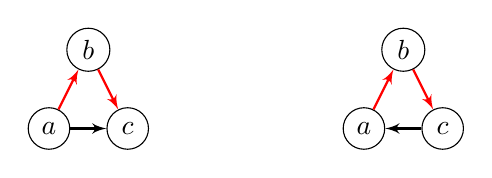
\begin{tikzpicture}
\tikzset{vertex/.style = {shape=circle,draw,minimum size=1.5em}}
\tikzset{edge/.style = {->,> = latex'}}
% vertices
\node[vertex] (a) at  (0,0) {$\!a\!$};
\node[vertex] (b) at  (0.5,1) {$\!b\!$};
\node[vertex] (c) at  (1,0) {$\!c\!$};

%edges
\draw[edge, thick][red] (a) to (b);
\draw[edge, thick] (a) to (c);
\draw[edge, thick][red] (b) to (c);

%\draw[edge] (a)  to[bend left] (a1);
%\draw[edge] (a1) to[bend left] (a);
%\path (a2) to node {\dots} (c);
%\node [shape=circle,minimum size=1.5em] (a3) at (4.5,0) {};
%\node [shape=circle,minimum size=1.5em] (c1) at (6.5,0) {};

\node[vertex] (d) at  (4,0) {$\!a\!$};
\node[vertex] (e) at  (4.5,1) {$\!b\!$};
\node[vertex] (f) at  (5,0) {$\!c\!$};

%edges
\draw[edge, thick][red] (d) to (e);
\draw[edge, thick] (f) to (d);
\draw[edge, thick][red] (e) to (f);

\end{tikzpicture}
\end{figure}

These tournaments represent the only two equivalence classes for $n=3$ tournaments: a cycle and a transitive tournament. While any combination of a cycle and transitive tournament would suffice to represent both equivalence classes, the tournaments chosen above have the interesting property of sharing two edges $ab$ and $bc$ (colored red). This property allows us to produce a short formula that admits both graphs:
\[
ab \land bc.
\]

This formula admits exactly one of the two labeled cycles and one of the six labeled transitive tournaments on 3 vertices, and does so with the fewest number of clauses. Therefore, $ab \land bc$ is a perfect, optimal isolator for $n=3$ tournaments.

Figure \ref{iso4} displays all 4 canonical representatives for $n=4$ tournaments. We note that once again all highlighted edges have the same edge labels across graphs, and all permutations of non-highlighted edges are present. So, a short formula that admits exactly the set of graphs in the figure is
\[
ab \land bc \land cd \land ad.
\]

While the optimal isolators for $n=3,4$ are comprised entirely of unit clauses, this pattern does not hold for $n=5$. Table \ref{tab:smallest_isolators_found} contains the number of unit and non-unit clauses for $n \le 7$.

\begin{figure}
\centering
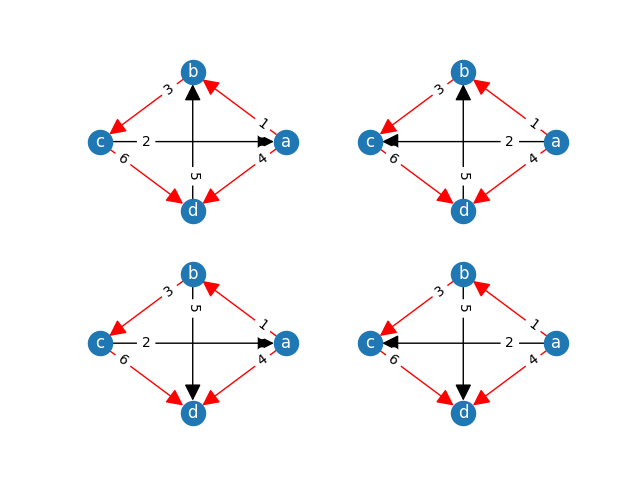
\includegraphics[width=0.4\textwidth]{iso_4.png}
\caption{All isomorphism class representatives admitted by a perfect, optimal isolator for 4-vertex tournaments. Red edges are edges fixed by unit clauses of the isolator, and the isolator has only unit clauses. Edge labels are the integers returned by the $\mathit{idx}$ function from the Arc Literal Numbering section.} \label{iso4}
\end{figure}

\subsection{Comparison of undirected graph and tournament isolators}

Although the majority of this work focuses on tournament isolators, there are many interesting parallels between undirected and tournament isolators. In an undirected context, the \emph{existence} of edge $(u,v)$ is denoted by the literal $uv$, while its nonexistence is denoted by the literal's negation $\lnot uv$.
Because edgeless and complete graphs are isomorphism classes for any $n$ in the undirected case, every clause of an undirected graph isolator containing only arc literals must contain at least one positive and one negative literal. These two graphs do not exist in the case of tournaments; the closest parallel is transitive tournaments. Unlike the set of $n$-vertex undirected graphs which contains exactly one empty graph and one complete graph with $n!$ automorphisms each, there are $n!$ isomorphic transitive tournaments on $n$ vertices. It is possible to select the particular transitive tournament $TT$ that an isolator admits by ensuring that at least one edge from $TT$ is present in each clause of the isolator. A simple way to do so is ensure each clause contains at least one edge $uv$ s.t. $u<v$ in vertex numbering. 

One consequence of undirected isolators requiring at least one positive and one negative literal per clause is that undirected isolators have no unit clauses. However, while negating all literals in an undirected isolator produces another undirected isolator (because the existence and non-existence of an edge is symmetric), there is no direct parallel to be found in tournaments as edge directionality does not have this property.

Another interesting difference between undirected graphs and tournaments is the low number of isomorphism classes for tournaments when $n$ is small (see table \ref{tab:smallest_isolators_found}). Intuitively, this happens because it is ``easier'' for tournaments to be isomorphic. The two options for the edge between vertices $u$ and $v$ in the undirected case are $uv$ existing or not existing. Crucially, an undirected graph $G$ will never be isomorphic to $G'$ constructed by adding or removing an edge of $G$, which is an operation that can be seen as ``flipping'' an edge to its other possibility. However, ``flipping'' an edge of a tournament $T$ by changing the edge's direction will produce $T' \simeq T$ iff the two vertices $u$ and $v$ of the flipped edge had the same edges to the rest of the graph (the isomorphism is via the permutation that swaps $u$ and $v$). Although this discrepancy exists for small $n$, the numbers of isomorphism classes for undirected graphs and tournaments are remarkably close for larger $n$ (see OEIS A000088, A00056 \cite{ref_oeis}). Therefore, we expect that perfect, optimal isolators for undirected graphs and tournaments will have similar numbers of clauses for larger $n$.

%Because it was desirable for these identifiers to be used directly as literals in a CNF formula, $idx_n(u,v)$ was constrained to satisfy certain properties.
\subsection{Arc Literal Numbering}
Each $uv$ must be assigned a corresponding integer to conform to the commonly used DIMACS CNF format.
To do so, we specify a function $idx_n(u,v)$ to map each possible arc $(u,v)$ in an $n$-vertex tournament to a unique integer identifier.  Because exactly one of $(u,v)$ and $(v,u)$ must exist for any two vertices $u,v$, $\mathit{idx}$ must satisfy $\mathit{idx}_n(u,v) = -\mathit{idx}_n(v,u)$. To facilitate isolator comparisons across different $n$, $\mathit{idx}$ also should satisfy the property that $\mathit{idx}_n(u,v) = \mathit{idx}_{n+1}(u,v)$. We therefore drop the subscript $n$ when referring to $\mathit{idx}_n(u,v) $ in the future, as its value does not depend on $n$. 

In particular, $\mathit{idx}$ is inductively defined as follows for an $n+1$-vertex tournament with vertices $v_1, v_2,,...v_n, v_{n+1}$. Let $K = n(n-1)/2$ be the largest output of $\mathit{idx}$ for an $n$-vertex tournament (implying base case $\mathit{idx}(v_1,v_2) = 1$ when $n=2$). Applying $\mathit{idx}$ to each of the arcs $(v_1,v_{n+1}), (v_2,v_{n+1}), ... (v_n, v_{n+1})$ yields $K+1, K+2,...,K+n$, respectively. All arcs not included in this definition are of the form $(v_w, v_u)$ where $w>u$, and are defined by the earlier mentioned constraint of $\mathit{idx}(u,v) = -\mathit{idx}(v,u)$.
%\hfill
%\begin{minipage}[t]{0.15\textwidth}
%  $ab, ac, cb$
%\end{minipage}
%\hfill
%\begin{minipage}[t]{0.15\textwidth}
%     $\begin{bmatrix}
%    0 & 1 & 1 \\
%    0 & 0 & 0 \\
%    0 & 1 & 0 \\
%    \end{bmatrix}$
%\end{minipage}

%Each edge in the edge list is directed from the first letter to the second, i.e. $ab$ represents the arc from $a$ to $b$. In the adjacency matrix, 





%Our main goal was to extend prior work \cite{ref_heule} with undirected graphs and generate optimal, perfect isolators for tournaments (complete, directed graphs). There were several places in which perfect isolator generation differed for tournaments.

%TBD: concrete examples section, move (un)directed comparison up here, move Figure 4 up, new figure for 3 verts
% add comparison about negation of isolator working vs not

%TBD: change image labels to ``a b c d'', make clear the two labeling schemes

% map file section might be good to split up: notation vs map specific stuff

% might need to revisit where to place map file generation

% make the explicit observation that there's no positive literal analog

% add in the proof sketch for Hamiltonian path, then cite


% begin{figure*} in order to put three figures in a row



%DONE

% small iso table: "iso classes" go second, could add # edges

% table captions go above tables

% caption text moved to text, then reference

%Kills -> Out (I chose excludes)

% B C D all one separate section

%E F G: section about units

% H I J additional techniques

% use capital C for clause, 'l' for literals. For every C_i, i in [1..k]...all clauses C_1... C_k

%switch order of (B C D) <-> (E F G)

%Erd\H{o}s

% in the sat encoding part, talk lots about "C_i, for i in [1..k]"

% Explain "we want exactly one", then give the encoding.

% use pi for permutation

% capital H in Hamiltonian path

%don't talk about map file in SAT encoding explanation

% figures: $n$ instead of plain text

% UNSAT -> unsatisfiable

% use proof environment when proving things

%idea: isolator background?

%@Jeremy do I need an extra sentence?


\section{Unit Clauses}

In practice, SAT solvers immediately reduce formulas with unit clauses to shorter formulas without units via unit propagation. Additionally, each unit clause reduces the size of the search space by a factor of 2. Therefore, it is practically useful to create isolators with as many units as possible. The following sections detail and analyze our various methods for creating isolators with many unit clauses.

\subsection{Provable Units}
While constructing smaller isolators using the techniques above, we opted to manually inspect our results and see what patterns they shared.  In doing so, we rediscovered a well-known fact from graph theory literature; every tournament contains a Hamiltonian path \cite{ref_tournament_book}. Proof sketch: inductively consider a length $n$ Hamiltonian path $v_1, v_2, ... v_n$ in an $n+1$-vertex tournament $G=(V,E)$. For the vertex $v_{n+1}$ not part of the path, in the case that either $(v_{n+1}, v_1)$ or $(v_n, v_{n+1})$ is in $E$, a length $n+1$ Hamiltonian path is formed. Otherwise, $(v_1, v_{n+1})$ and $(v_{n+1}, v_{n})$ are in $E$ and thus there must exist consecutive vertices $v_i,v_{i+1}$ in the Hamiltonian path such that arcs $(v_i,v_{n+1})$ and $(v_{n+1},v_{i+1})$ are in $E$. In this case, the sequence $v_1,v_2,...v_i, v_{n+1}, v_{i+1},...v_n$ forms a length $n+1$ Hamiltonian path. As a result of this property, a set of unit clauses describing a Hamiltonian path on an $n$-vertex tournament is always a valid $n$-vertex isolator.

%\begin{proof}
%Proceed by induction.  The statement is trivial for 1- and 2- vertex tournaments, since in the former the empty path is Hamiltonian and in the latter the sole edge is the path.  Now, given an $m$-length path in a tournament for $2 \le m < n-1$, argue that an $m+1$-length path exists.

%Label the vertices on the given path by $1$ through $m+1$, and since $m+1 < n$ there exists some other vertex $a$.  If there is an edge from $a$ to $1$ or $m+1$ to $a$, then we can trivially extend the path to include $a$, so take the other case where there is an edge from $1$ to $a$ and an edge from $a$ to $m+1$.  Consider the smallest $1 \le i \le m+1$ such that there is an edge from $a$ to $i$.  Clearly $i > 1$ as there is an edge from $1$ to $a$, and clearly $i$ is well-defined since the set of $i$ where there is an edge from $a$ to $i$ is nonempty as it contains $m+1$.  Then, we have that $i-1 \ge 1$, and furthermore there is no edge from $a$ to $i-1$, so there is an edge from $i-1$ to $a$.  Therefore, we can take $i-2$ steps on the original path from vertex $1$ to vertex $i-1$, one step from $i-1$ to $a$, one step from $a$ to $i$, and $m+1-i$ steps on the original path from vertex $i$ to vertex $m+1$.  This new path has length $(i-2) + (1) + (1) + (m+1-i) = m+1$, completing the induction step and thus the proof.  $\square$
%\end{proof}

%It is worth noting that we do not have a proof that it is always possible to extend an encoded Hamiltonian path to an \textit{optimal} isolator.  However, building off a set of units can make searching for compact isolators much more efficient. In particular, we modified our map-file generation to optionally ignore graphs that are not admitted by a given set of units. Including these units reduces the map file size and generation time by a factor of $2^{n-1}$, which makes map file-based approaches still viable for up to $n = 8$.

%Given the utility of unit clauses in isolators, a natural next question would be: can we bound the number of units in $n$-vertex isolators, either strictly or asymptotically? 
Given the utility of unit clauses in isolators, it is natural to ask how many units there can possibly be in an $n$-vertex isolator. As it turns out, there is a long-known result from graph theory that implies that asymptotically there are at most $O(n\log n)$ units possible. By the orbit-stabilizer theorem, the size of the equivalence class of a graph $G$ on $n$ vertices is $\frac{n!}{|Aut(G)|}$, where $Aut(G)$ is the set of distinct automorphisms of $G$. In 1963 Erd\H{o}s and R{\'e}nyi proved that as $n$ approaches infinity, the proportion of undirected graphs of size $n$ with with nontrivial automorphisms approaches 0 \cite{ref_asymmetric}. The same result for tournaments directly follows. Therefore, a proportion of tournaments approaching 1 has equivalence classes of size $n!$, so the asymptotic number of equivalence classes is
\[
\frac{2^{n \choose 2}}{n!} \in \Theta(\frac{2^{n \choose 2}}{2^{n\log n}}) = \Theta(2^{{n \choose 2} - n\log n}).
\]

An isolator with $k$ unit clauses for $n$-vertex graphs admits at most $2^{{n \choose 2} - k}$ equivalence class representatives, so in order to admit at least one member of each equivalence class (by the definition of an isolator), the number of units in an isolator must also be asymptotically upper-bounded by $n \log n$.

In the next section, we provide a procedure that achieves this bound.

\subsection{TT-fixing}

%We seek to prove that at least $n\log{n}$???(placeholder) units can be part of an isolator for $n$-vertex tournaments.  
%If a $TT_k$ is known to exist within every member of the class of $n$-vertex tournaments,
In situations where we know that every member of the class of $n$-vertex tournaments contains a $TT_k$ (a transitive tournament of size k), we also know that every equivalence class must contain a member with the tournament fixed in some arbitrary position and orientation (i.e. vertices $1$ through $k$ in ascending order). Therefore, any formula that \emph{fixes} (i.e. asserts the existence of) a $TT_k$ on the class of $n$-vertex tournaments is a valid isolator. Because the remaining subset of $n-k$ non-fixed vertices also forms a tournament, further knowledge about the existence of a transitive tournament within the remaining $n-k$ vertices can be used to fix (via units) another transitive tournament within the $n-k$ vertex subtournament. This procedure can be repeated until all vertices of the original tournament are part of some fixed transitive subtournament. Tournament Ramsey numbers provide exactly the required information about the existence of a transitive subtournament. In fact, tournament Ramsey numbers (when known) provide the \textit{largest} transitive subtournament guaranteed to exist in a tournament of a given size. Therefore, tournament Ramsey numbers (as well as upper bounds, which exist for arbitrarily large $n$) can be used to iteratively construct large sets of unit clauses for tournament isolators: we will refer to this process as TT-fixing.

%\textbf{add algorithm TBD}

%\newcommand*\circled[1]{\tikz[baseline=(char.base)]{
%            \node[fill=black,shape=circle,draw,inner sep=1pt] (char) {\textcolor{white}{#1}};}}
%\newcommand{\zero}{ 0}
%\newcommand{\one}{ \circled{1}}


\begin{figure}
$$\left[
\begin{array}{c@{\,}c@{\,}c@{\,}c@{\,}c@{\,}c@{\,}c@{\,}c@{\,}c@{\,}c@{\,}c@{\,}c@{\,}c@{\,}c@{\,}c@{\,}c}
\zero & \one & \one & \one & \one & \none & \none & \none & \none & \none & \none & \none & \none & \none & \none & \none\\
\zero & \zero & \one & \one & \one & \none & \none & \none & \none & \none & \none & \none & \none & \none & \none & \none\\
\zero & \zero & \zero & \one & \one & \none & \none & \none & \none & \none & \none & \none & \none & \none & \none & \none\\
\zero & \zero & \zero & \zero & \one & \none & \none & \none & \none & \none & \none & \none & \none & \none & \none & \none\\
\zero & \zero & \zero & \zero & \zero & \none & \none & \none & \none & \none & \none & \none & \none & \none & \none & \none\\
\none & \none & \none & \none & \none & \zero & \one & \one & \one & \none & \none & \none & \none & \none & \none & \none\\
\none & \none & \none & \none & \none & \zero & \zero & \one & \one & \none & \none & \none & \none & \none & \none & \none\\
\none & \none & \none & \none & \none & \zero & \zero & \zero & \one & \none & \none & \none & \none & \none & \none & \none\\
\none & \none & \none & \none & \none & \zero & \zero & \zero & \zero & \none & \none & \none & \none & \none & \none & \none\\
\none & \none & \none & \none & \none & \none & \none & \none & \none & \zero & \one & \one & \none & \none & \none & \none\\
\none & \none & \none & \none & \none & \none & \none & \none & \none & \zero & \zero & \one & \none & \none & \none & \none\\
\none & \none & \none & \none & \none & \none & \none & \none & \none & \zero & \zero & \zero & \none & \none & \none & \none\\
\none & \none & \none & \none & \none & \none & \none & \none & \none & \none & \none & \none & \zero & \one & \one & \none\\
\none & \none & \none & \none & \none & \none & \none & \none & \none & \none & \none & \none & \zero & \zero & \one & \none\\
\none & \none & \none & \none & \none & \none & \none & \none & \none & \none & \none & \none & \zero & \zero & \zero & \none\\
\none & \none & \none & \none & \none & \none & \none & \none & \none & \none & \none & \none & \none & \none & \none & \zero\\
\end{array}
\right]$$
\end{figure}

% add algorithm
% add diagram

%Instead of using Ramsey numbers to provide a guarantee on the existence of a transitive tournament, one simpler procedure for generating isolator units for $n$-vertex tournaments is as follows: for all $0 \le i < n/2 -1$, vertices $2i$ and $2i+1$ are symmetric with respect to the remaining vertices. So, all such symmetries can be broken by adding the units corresponding to the arcs $(2i, 2i+1)$. However, such a procedure yields approximately $n/2$ units, which is quite far from the $n\log n$ bound. The complexity of TT-fixing is justified by the number of units it provides, which we now show to be $\Theta(n\log n)$.

% $R(k) \leq 2R(k-1)$, which implies 


\subsection{TT-fixing gives $\Theta(n\log n)$ units}
Let $units(n)$ be the function that returns the number of units that can be added to an isolator when using the TT-fixing method on $n$-vertex tournaments. Our goal is to prove a lower bound on $units(n)$. Unfortunately, exact tournament Ramsey numbers are non-trivial to calculate (only up to $R(6) = 28$ is known). However, from Erd\H{o}s and Moser  we have that $R(k) \leq 2^{k-1}$ \cite{ref_erdos_ramsey_bounds}, i.e. that a $TT_{k}$ must exist when considering any tournament on $2^{k-1}$ or more vertices. Erd\H{o}s and Moser's bound can thus be used with TT-fixing to lower-bound $units(n)$.

We claim that $units(n) \geq \sum\limits_{i=1}^n \frac{1}{2} \lfloor \log_2(i) \rfloor$. We proceed via induction, with step $n$ depending on step $n-k$, with $k=\lfloor \log_2(n)\rfloor + 1$. The proposition is true for $n=1$ because $0 \geq 0$, $n=2$ because $ 1 \geq 0.5$.  By definition of TT-fixing, for a graph with $n$ vertices we have 

\begin{equation}\label{unitsndef}
units(n) = \frac{k(k-1)}{2}  + units(n-k).
\end{equation} 

By the inductive hypothesis,

 \begin{equation}\label{unitsIH}
 units(n-k) \geq \sum\limits_{i=1}^{n-k} \lfloor \log_2(i)\rfloor/2.
 \end{equation}
 
 Next, we have that 
 \begin{align}
  k\frac{k-1}{2} &= k \lfloor \log_2(n)\rfloor/2 \nonumber \\
   &= \sum\limits_{i=n-k+1}^{n} \lfloor \log_2(n)\rfloor/2 \nonumber \\
  &\geq \sum\limits_{i=n-k+1}^{n} \lfloor \log_2(i)\rfloor/2  \label{unitsk}.
 \end{align}
 
 Combining lower bounds (\ref{unitsIH}) and (\ref{unitsk}) for the terms of \cref{unitsndef} completes the proof: 
 \begin{align}
 units(n) &= \frac{k(k-1)}{2} + units(n-k) \nonumber \\
 &\geq \sum\limits_{i=n-k+1}^{n} \lfloor \log_2(i)\rfloor/2 + \sum\limits_{i=1}^{n-k} \lfloor \log_2(i)\rfloor/2 \\
 &= \sum\limits_{i=1}^{n} \lfloor \log_2(i)\rfloor/2.
 \end{align}
 
 This inequality result directly implies the asymptotic $n\log n$ bound, because $\log_2(n!) \in \Theta(n \log n)$. 

\begin{figure}
\centering
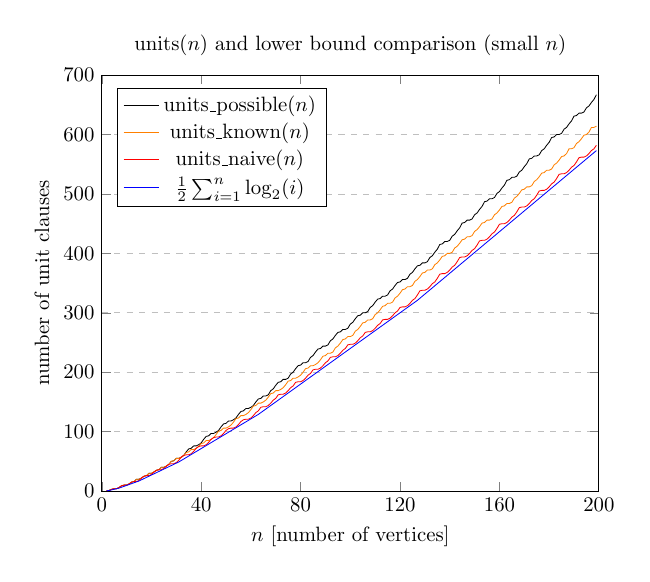
\begin{tikzpicture}[scale = 0.75]
\begin{axis}[
    title={units($n$) and lower bound comparison (small $n$)},
    xlabel={$n$ [number of vertices]},
    ylabel={number of unit clauses},
    xmin=0, xmax=200,
    ymin=0, ymax=700,
    xtick={0,40,80,120,160,200},
    ytick={0,100,200,300,400,500,600,700},
    legend pos=north west,
    ymajorgrids=true,
    grid style=dashed,
]

\addplot[
    color=black,
    ]
    coordinates {
(2,1)(3,1)(4,3)(5,4)(6,4)(7,6)(8,9)(9,10)(10,10)(11,12)(12,15)(13,16)(14,20)(15,20)(16,22)(17,25)(18,26)(19,30)(20,30)(21,32)(22,35)(23,36)(24,40)(25,40)(26,42)(27,45)(28,50)(29,51)(30,55)(31,55)(32,57)(33,60)(34,66)(35,71)(36,72)(37,76)(38,76)(39,78)(40,81)(41,87)(42,92)(43,93)(44,97)(45,97)(46,99)(47,102)(48,108)(49,113)(50,114)(51,118)(52,118)(53,120)(54,123)(55,129)(56,134)(57,135)(58,139)(59,139)(60,141)(61,144)(62,150)(63,155)(64,156)(65,160)(66,160)(67,162)(68,169)(69,172)(70,178)(71,183)(72,184)(73,188)(74,188)(75,190)(76,197)(77,200)(78,206)(79,211)(80,212)(81,216)(82,216)(83,218)(84,225)(85,228)(86,234)(87,239)(88,240)(89,244)(90,244)(91,246)(92,253)(93,256)(94,262)(95,267)(96,268)(97,272)(98,272)(99,274)(100,281)(101,284)(102,290)(103,295)(104,296)(105,300)(106,300)(107,302)(108,309)(109,312)(110,318)(111,323)(112,324)(113,328)(114,328)(115,330)(116,337)(117,340)(118,346)(119,351)(120,352)(121,356)(122,356)(123,358)(124,365)(125,368)(126,374)(127,379)(128,380)(129,384)(130,384)(131,386)(132,393)(133,396)(134,402)(135,407)(136,415)(137,416)(138,420)(139,420)(140,422)(141,429)(142,432)(143,438)(144,443)(145,451)(146,452)(147,456)(148,456)(149,458)(150,465)(151,468)(152,474)(153,479)(154,487)(155,488)(156,492)(157,492)(158,494)(159,501)(160,504)(161,510)(162,515)(163,523)(164,524)(165,528)(166,528)(167,530)(168,537)(169,540)(170,546)(171,551)(172,559)(173,560)(174,564)(175,564)(176,566)(177,573)(178,576)(179,582)(180,587)(181,595)(182,596)(183,600)(184,600)(185,602)(186,609)(187,612)(188,618)(189,623)(190,631)(191,632)(192,636)(193,636)(194,638)(195,645)(196,648)(197,654)(198,659)(199,667)
    };
    \addlegendentry{units\_possible($n$)}

\addplot[
    color=orange,
    ]
    coordinates {
(2,1)(3,1)(4,3)(5,4)(6,4)(7,6)(8,9)(9,10)(10,10)(11,12)(12,15)(13,16)(14,20)(15,20)(16,22)(17,25)(18,26)(19,30)(20,30)(21,32)(22,35)(23,36)(24,40)(25,40)(26,42)(27,45)(28,50)(29,51)(30,55)(31,55)(32,57)(33,60)(34,65)(35,66)(36,70)(37,70)(38,72)(39,75)(40,80)(41,81)(42,85)(43,85)(44,87)(45,90)(46,95)(47,101)(48,102)(49,106)(50,106)(51,108)(52,111)(53,116)(54,122)(55,123)(56,127)(57,127)(58,129)(59,132)(60,137)(61,143)(62,144)(63,148)(64,148)(65,150)(66,153)(67,158)(68,164)(69,165)(70,169)(71,169)(72,171)(73,174)(74,179)(75,185)(76,186)(77,190)(78,190)(79,192)(80,195)(81,200)(82,206)(83,207)(84,211)(85,211)(86,213)(87,216)(88,221)(89,227)(90,228)(91,232)(92,232)(93,234)(94,241)(95,244)(96,249)(97,255)(98,256)(99,260)(100,260)(101,262)(102,269)(103,272)(104,277)(105,283)(106,284)(107,288)(108,288)(109,290)(110,297)(111,300)(112,305)(113,311)(114,312)(115,316)(116,316)(117,318)(118,325)(119,328)(120,333)(121,339)(122,340)(123,344)(124,344)(125,346)(126,353)(127,356)(128,361)(129,367)(130,368)(131,372)(132,372)(133,374)(134,381)(135,384)(136,389)(137,395)(138,396)(139,400)(140,400)(141,402)(142,409)(143,412)(144,417)(145,423)(146,424)(147,428)(148,428)(149,430)(150,437)(151,440)(152,445)(153,451)(154,452)(155,456)(156,456)(157,458)(158,465)(159,468)(160,473)(161,479)(162,480)(163,484)(164,484)(165,486)(166,493)(167,496)(168,501)(169,507)(170,508)(171,512)(172,512)(173,514)(174,521)(175,524)(176,529)(177,535)(178,536)(179,540)(180,540)(181,542)(182,549)(183,552)(184,557)(185,563)(186,564)(187,568)(188,576)(189,576)(190,578)(191,585)(192,588)(193,593)(194,599)(195,600)(196,604)(197,612)(198,612)(199,614)
    };
    \addlegendentry{units\_known($n$)}

\addplot[
    color=red,
    ]
    coordinates {
(2,1)(3,1)(4,3)(5,4)(6,4)(7,6)(8,9)(9,10)(10,10)(11,12)(12,15)(13,16)(14,16)(15,18)(16,22)(17,25)(18,26)(19,26)(20,28)(21,32)(22,35)(23,36)(24,36)(25,38)(26,42)(27,45)(28,46)(29,46)(30,48)(31,52)(32,57)(33,60)(34,61)(35,61)(36,63)(37,67)(38,72)(39,75)(40,76)(41,76)(42,78)(43,82)(44,87)(45,90)(46,91)(47,91)(48,93)(49,97)(50,102)(51,105)(52,106)(53,106)(54,108)(55,112)(56,117)(57,120)(58,121)(59,121)(60,123)(61,127)(62,132)(63,135)(64,141)(65,142)(66,142)(67,144)(68,148)(69,153)(70,156)(71,162)(72,163)(73,163)(74,165)(75,169)(76,174)(77,177)(78,183)(79,184)(80,184)(81,186)(82,190)(83,195)(84,198)(85,204)(86,205)(87,205)(88,207)(89,211)(90,216)(91,219)(92,225)(93,226)(94,226)(95,228)(96,232)(97,237)(98,240)(99,246)(100,247)(101,247)(102,249)(103,253)(104,258)(105,261)(106,267)(107,268)(108,268)(109,270)(110,274)(111,279)(112,282)(113,288)(114,289)(115,289)(116,291)(117,295)(118,300)(119,303)(120,309)(121,310)(122,310)(123,312)(124,316)(125,321)(126,324)(127,330)(128,337)(129,338)(130,338)(131,340)(132,344)(133,349)(134,352)(135,358)(136,365)(137,366)(138,366)(139,368)(140,372)(141,377)(142,380)(143,386)(144,393)(145,394)(146,394)(147,396)(148,400)(149,405)(150,408)(151,414)(152,421)(153,422)(154,422)(155,424)(156,428)(157,433)(158,436)(159,442)(160,449)(161,450)(162,450)(163,452)(164,456)(165,461)(166,464)(167,470)(168,477)(169,478)(170,478)(171,480)(172,484)(173,489)(174,492)(175,498)(176,505)(177,506)(178,506)(179,508)(180,512)(181,517)(182,520)(183,526)(184,533)(185,534)(186,534)(187,536)(188,540)(189,545)(190,548)(191,554)(192,561)(193,562)(194,562)(195,564)(196,568)(197,573)(198,576)(199,582)
    };
    \addlegendentry{units\_naive($n$)}

\addplot[
    color=blue,
    ]
    coordinates {
    (2,0.5)(3,1.0)(4,2.0)(5,3.0)(6,4.0)(7,5.0)(8,6.5)(9,8.0)(10,9.5)(11,11.0)(12,12.5)(13,14.0)(14,15.5)(15,17.0)(16,19.0)(17,21.0)(18,23.0)(19,25.0)(20,27.0)(21,29.0)(22,31.0)(23,33.0)(24,35.0)(25,37.0)(26,39.0)(27,41.0)(28,43.0)(29,45.0)(30,47.0)(31,49.0)(32,51.5)(33,54.0)(34,56.5)(35,59.0)(36,61.5)(37,64.0)(38,66.5)(39,69.0)(40,71.5)(41,74.0)(42,76.5)(43,79.0)(44,81.5)(45,84.0)(46,86.5)(47,89.0)(48,91.5)(49,94.0)(50,96.5)(51,99.0)(52,101.5)(53,104.0)(54,106.5)(55,109.0)(56,111.5)(57,114.0)(58,116.5)(59,119.0)(60,121.5)(61,124.0)(62,126.5)(63,129.0)(64,132.0)(65,135.0)(66,138.0)(67,141.0)(68,144.0)(69,147.0)(70,150.0)(71,153.0)(72,156.0)(73,159.0)(74,162.0)(75,165.0)(76,168.0)(77,171.0)(78,174.0)(79,177.0)(80,180.0)(81,183.0)(82,186.0)(83,189.0)(84,192.0)(85,195.0)(86,198.0)(87,201.0)(88,204.0)(89,207.0)(90,210.0)(91,213.0)(92,216.0)(93,219.0)(94,222.0)(95,225.0)(96,228.0)(97,231.0)(98,234.0)(99,237.0)(100,240.0)(101,243.0)(102,246.0)(103,249.0)(104,252.0)(105,255.0)(106,258.0)(107,261.0)(108,264.0)(109,267.0)(110,270.0)(111,273.0)(112,276.0)(113,279.0)(114,282.0)(115,285.0)(116,288.0)(117,291.0)(118,294.0)(119,297.0)(120,300.0)(121,303.0)(122,306.0)(123,309.0)(124,312.0)(125,315.0)(126,318.0)(127,321.0)(128,324.5)(129,328.0)(130,331.5)(131,335.0)(132,338.5)(133,342.0)(134,345.5)(135,349.0)(136,352.5)(137,356.0)(138,359.5)(139,363.0)(140,366.5)(141,370.0)(142,373.5)(143,377.0)(144,380.5)(145,384.0)(146,387.5)(147,391.0)(148,394.5)(149,398.0)(150,401.5)(151,405.0)(152,408.5)(153,412.0)(154,415.5)(155,419.0)(156,422.5)(157,426.0)(158,429.5)(159,433.0)(160,436.5)(161,440.0)(162,443.5)(163,447.0)(164,450.5)(165,454.0)(166,457.5)(167,461.0)(168,464.5)(169,468.0)(170,471.5)(171,475.0)(172,478.5)(173,482.0)(174,485.5)(175,489.0)(176,492.5)(177,496.0)(178,499.5)(179,503.0)(180,506.5)(181,510.0)(182,513.5)(183,517.0)(184,520.5)(185,524.0)(186,527.5)(187,531.0)(188,534.5)(189,538.0)(190,541.5)(191,545.0)(192,548.5)(193,552.0)(194,555.5)(195,559.0)(196,562.5)(197,566.0)(198,569.5)(199,573.0)
    };
    \addlegendentry{$\frac{1}{2}\sum_{i=1}^n \log_2(i)$}
    
\end{axis}
\end{tikzpicture}
\caption{A visual depiction of how the number of unit clauses produced by TT-fixing grows under different assumptions about Ramsey numbers.} 
\label{pracunits}
\end{figure}

%\begin{figure}
%\centering
%\begin{tikzpicture}[scale=0.75]
%\begin{axis}[
%    title={units($n$) and lower bound comparison (large $n$)},
%    xlabel={$n$ [number of vertices]},
%    ylabel={number of unit clauses},
%    xmin=0, xmax=100000,
%    ymin=0, ymax=800000,
%    xtick={0,20000,40000,60000,80000,100000},
%    ytick={0,100000,200000,300000,400000,500000,600000,700000,800000},
%    legend pos=north west,
%    ymajorgrids=true,
%    grid style=dashed,
%]
%
%\addplot[
%    color=blue,
%    ]
%    coordinates {
%(2,0.5)(101,243.0)(200,576.5)(299,945.0)(398,1341.0)(497,1737.0)(596,2175.5)(695,2621.0)(794,3066.5)(893,3512.0)(992,3957.5)(1091,4437.0)(1190,4932.0)(1289,5427.0)(1388,5922.0)(1487,6417.0)(1586,6912.0)(1685,7407.0)(1784,7902.0)(1883,8397.0)(1982,8892.0)(2081,9404.0)(2180,9948.5)(2279,10493.0)(2378,11037.5)(2477,11582.0)(2576,12126.5)(2675,12671.0)(2774,13215.5)(2873,13760.0)(2972,14304.5)(3071,14849.0)(3170,15393.5)(3269,15938.0)(3368,16482.5)(3467,17027.0)(3566,17571.5)(3665,18116.0)(3764,18660.5)(3863,19205.0)(3962,19749.5)(4061,20294.0)(4160,20871.0)(4259,21465.0)(4358,22059.0)(4457,22653.0)(4556,23247.0)(4655,23841.0)(4754,24435.0)(4853,25029.0)(4952,25623.0)(5051,26217.0)(5150,26811.0)(5249,27405.0)(5348,27999.0)(5447,28593.0)(5546,29187.0)(5645,29781.0)(5744,30375.0)(5843,30969.0)(5942,31563.0)(6041,32157.0)(6140,32751.0)(6239,33345.0)(6338,33939.0)(6437,34533.0)(6536,35127.0)(6635,35721.0)(6734,36315.0)(6833,36909.0)(6932,37503.0)(7031,38097.0)(7130,38691.0)(7229,39285.0)(7328,39879.0)(7427,40473.0)(7526,41067.0)(7625,41661.0)(7724,42255.0)(7823,42849.0)(7922,43443.0)(8021,44037.0)(8120,44631.0)(8219,45239.0)(8318,45882.5)(8417,46526.0)(8516,47169.5)(8615,47813.0)(8714,48456.5)(8813,49100.0)(8912,49743.5)(9011,50387.0)(9110,51030.5)(9209,51674.0)(9308,52317.5)(9407,52961.0)(9506,53604.5)(9605,54248.0)(9704,54891.5)(9803,55535.0)(9902,56178.5)(10001,56822.0)(10100,57465.5)(10199,58109.0)(10298,58752.5)(10397,59396.0)(10496,60039.5)(10595,60683.0)(10694,61326.5)(10793,61970.0)(10892,62613.5)(10991,63257.0)(11090,63900.5)(11189,64544.0)(11288,65187.5)(11387,65831.0)(11486,66474.5)(11585,67118.0)(11684,67761.5)(11783,68405.0)(11882,69048.5)(11981,69692.0)(12080,70335.5)(12179,70979.0)(12278,71622.5)(12377,72266.0)(12476,72909.5)(12575,73553.0)(12674,74196.5)(12773,74840.0)(12872,75483.5)(12971,76127.0)(13070,76770.5)(13169,77414.0)(13268,78057.5)(13367,78701.0)(13466,79344.5)(13565,79988.0)(13664,80631.5)(13763,81275.0)(13862,81918.5)(13961,82562.0)(14060,83205.5)(14159,83849.0)(14258,84492.5)(14357,85136.0)(14456,85779.5)(14555,86423.0)(14654,87066.5)(14753,87710.0)(14852,88353.5)(14951,88997.0)(15050,89640.5)(15149,90284.0)(15248,90927.5)(15347,91571.0)(15446,92214.5)(15545,92858.0)(15644,93501.5)(15743,94145.0)(15842,94788.5)(15941,95432.0)(16040,96075.5)(16139,96719.0)(16238,97362.5)(16337,98006.0)(16436,98676.0)(16535,99369.0)(16634,100062.0)(16733,100755.0)(16832,101448.0)(16931,102141.0)(17030,102834.0)(17129,103527.0)(17228,104220.0)(17327,104913.0)(17426,105606.0)(17525,106299.0)(17624,106992.0)(17723,107685.0)(17822,108378.0)(17921,109071.0)(18020,109764.0)(18119,110457.0)(18218,111150.0)(18317,111843.0)(18416,112536.0)(18515,113229.0)(18614,113922.0)(18713,114615.0)(18812,115308.0)(18911,116001.0)(19010,116694.0)(19109,117387.0)(19208,118080.0)(19307,118773.0)(19406,119466.0)(19505,120159.0)(19604,120852.0)(19703,121545.0)(19802,122238.0)(19901,122931.0)(20000,123624.0)(20099,124317.0)(20198,125010.0)(20297,125703.0)(20396,126396.0)(20495,127089.0)(20594,127782.0)(20693,128475.0)(20792,129168.0)(20891,129861.0)(20990,130554.0)(21089,131247.0)(21188,131940.0)(21287,132633.0)(21386,133326.0)(21485,134019.0)(21584,134712.0)(21683,135405.0)(21782,136098.0)(21881,136791.0)(21980,137484.0)(22079,138177.0)(22178,138870.0)(22277,139563.0)(22376,140256.0)(22475,140949.0)(22574,141642.0)(22673,142335.0)(22772,143028.0)(22871,143721.0)(22970,144414.0)(23069,145107.0)(23168,145800.0)(23267,146493.0)(23366,147186.0)(23465,147879.0)(23564,148572.0)(23663,149265.0)(23762,149958.0)(23861,150651.0)(23960,151344.0)(24059,152037.0)(24158,152730.0)(24257,153423.0)(24356,154116.0)(24455,154809.0)(24554,155502.0)(24653,156195.0)(24752,156888.0)(24851,157581.0)(24950,158274.0)(25049,158967.0)(25148,159660.0)(25247,160353.0)(25346,161046.0)(25445,161739.0)(25544,162432.0)(25643,163125.0)(25742,163818.0)(25841,164511.0)(25940,165204.0)(26039,165897.0)(26138,166590.0)(26237,167283.0)(26336,167976.0)(26435,168669.0)(26534,169362.0)(26633,170055.0)(26732,170748.0)(26831,171441.0)(26930,172134.0)(27029,172827.0)(27128,173520.0)(27227,174213.0)(27326,174906.0)(27425,175599.0)(27524,176292.0)(27623,176985.0)(27722,177678.0)(27821,178371.0)(27920,179064.0)(28019,179757.0)(28118,180450.0)(28217,181143.0)(28316,181836.0)(28415,182529.0)(28514,183222.0)(28613,183915.0)(28712,184608.0)(28811,185301.0)(28910,185994.0)(29009,186687.0)(29108,187380.0)(29207,188073.0)(29306,188766.0)(29405,189459.0)(29504,190152.0)(29603,190845.0)(29702,191538.0)(29801,192231.0)(29900,192924.0)(29999,193617.0)(30098,194310.0)(30197,195003.0)(30296,195696.0)(30395,196389.0)(30494,197082.0)(30593,197775.0)(30692,198468.0)(30791,199161.0)(30890,199854.0)(30989,200547.0)(31088,201240.0)(31187,201933.0)(31286,202626.0)(31385,203319.0)(31484,204012.0)(31583,204705.0)(31682,205398.0)(31781,206091.0)(31880,206784.0)(31979,207477.0)(32078,208170.0)(32177,208863.0)(32276,209556.0)(32375,210249.0)(32474,210942.0)(32573,211635.0)(32672,212328.0)(32771,213023.0)(32870,213765.5)(32969,214508.0)(33068,215250.5)(33167,215993.0)(33266,216735.5)(33365,217478.0)(33464,218220.5)(33563,218963.0)(33662,219705.5)(33761,220448.0)(33860,221190.5)(33959,221933.0)(34058,222675.5)(34157,223418.0)(34256,224160.5)(34355,224903.0)(34454,225645.5)(34553,226388.0)(34652,227130.5)(34751,227873.0)(34850,228615.5)(34949,229358.0)(35048,230100.5)(35147,230843.0)(35246,231585.5)(35345,232328.0)(35444,233070.5)(35543,233813.0)(35642,234555.5)(35741,235298.0)(35840,236040.5)(35939,236783.0)(36038,237525.5)(36137,238268.0)(36236,239010.5)(36335,239753.0)(36434,240495.5)(36533,241238.0)(36632,241980.5)(36731,242723.0)(36830,243465.5)(36929,244208.0)(37028,244950.5)(37127,245693.0)(37226,246435.5)(37325,247178.0)(37424,247920.5)(37523,248663.0)(37622,249405.5)(37721,250148.0)(37820,250890.5)(37919,251633.0)(38018,252375.5)(38117,253118.0)(38216,253860.5)(38315,254603.0)(38414,255345.5)(38513,256088.0)(38612,256830.5)(38711,257573.0)(38810,258315.5)(38909,259058.0)(39008,259800.5)(39107,260543.0)(39206,261285.5)(39305,262028.0)(39404,262770.5)(39503,263513.0)(39602,264255.5)(39701,264998.0)(39800,265740.5)(39899,266483.0)(39998,267225.5)(40097,267968.0)(40196,268710.5)(40295,269453.0)(40394,270195.5)(40493,270938.0)(40592,271680.5)(40691,272423.0)(40790,273165.5)(40889,273908.0)(40988,274650.5)(41087,275393.0)(41186,276135.5)(41285,276878.0)(41384,277620.5)(41483,278363.0)(41582,279105.5)(41681,279848.0)(41780,280590.5)(41879,281333.0)(41978,282075.5)(42077,282818.0)(42176,283560.5)(42275,284303.0)(42374,285045.5)(42473,285788.0)(42572,286530.5)(42671,287273.0)(42770,288015.5)(42869,288758.0)(42968,289500.5)(43067,290243.0)(43166,290985.5)(43265,291728.0)(43364,292470.5)(43463,293213.0)(43562,293955.5)(43661,294698.0)(43760,295440.5)(43859,296183.0)(43958,296925.5)(44057,297668.0)(44156,298410.5)(44255,299153.0)(44354,299895.5)(44453,300638.0)(44552,301380.5)(44651,302123.0)(44750,302865.5)(44849,303608.0)(44948,304350.5)(45047,305093.0)(45146,305835.5)(45245,306578.0)(45344,307320.5)(45443,308063.0)(45542,308805.5)(45641,309548.0)(45740,310290.5)(45839,311033.0)(45938,311775.5)(46037,312518.0)(46136,313260.5)(46235,314003.0)(46334,314745.5)(46433,315488.0)(46532,316230.5)(46631,316973.0)(46730,317715.5)(46829,318458.0)(46928,319200.5)(47027,319943.0)(47126,320685.5)(47225,321428.0)(47324,322170.5)(47423,322913.0)(47522,323655.5)(47621,324398.0)(47720,325140.5)(47819,325883.0)(47918,326625.5)(48017,327368.0)(48116,328110.5)(48215,328853.0)(48314,329595.5)(48413,330338.0)(48512,331080.5)(48611,331823.0)(48710,332565.5)(48809,333308.0)(48908,334050.5)(49007,334793.0)(49106,335535.5)(49205,336278.0)(49304,337020.5)(49403,337763.0)(49502,338505.5)(49601,339248.0)(49700,339990.5)(49799,340733.0)(49898,341475.5)(49997,342218.0)(50096,342960.5)(50195,343703.0)(50294,344445.5)(50393,345188.0)(50492,345930.5)(50591,346673.0)(50690,347415.5)(50789,348158.0)(50888,348900.5)(50987,349643.0)(51086,350385.5)(51185,351128.0)(51284,351870.5)(51383,352613.0)(51482,353355.5)(51581,354098.0)(51680,354840.5)(51779,355583.0)(51878,356325.5)(51977,357068.0)(52076,357810.5)(52175,358553.0)(52274,359295.5)(52373,360038.0)(52472,360780.5)(52571,361523.0)(52670,362265.5)(52769,363008.0)(52868,363750.5)(52967,364493.0)(53066,365235.5)(53165,365978.0)(53264,366720.5)(53363,367463.0)(53462,368205.5)(53561,368948.0)(53660,369690.5)(53759,370433.0)(53858,371175.5)(53957,371918.0)(54056,372660.5)(54155,373403.0)(54254,374145.5)(54353,374888.0)(54452,375630.5)(54551,376373.0)(54650,377115.5)(54749,377858.0)(54848,378600.5)(54947,379343.0)(55046,380085.5)(55145,380828.0)(55244,381570.5)(55343,382313.0)(55442,383055.5)(55541,383798.0)(55640,384540.5)(55739,385283.0)(55838,386025.5)(55937,386768.0)(56036,387510.5)(56135,388253.0)(56234,388995.5)(56333,389738.0)(56432,390480.5)(56531,391223.0)(56630,391965.5)(56729,392708.0)(56828,393450.5)(56927,394193.0)(57026,394935.5)(57125,395678.0)(57224,396420.5)(57323,397163.0)(57422,397905.5)(57521,398648.0)(57620,399390.5)(57719,400133.0)(57818,400875.5)(57917,401618.0)(58016,402360.5)(58115,403103.0)(58214,403845.5)(58313,404588.0)(58412,405330.5)(58511,406073.0)(58610,406815.5)(58709,407558.0)(58808,408300.5)(58907,409043.0)(59006,409785.5)(59105,410528.0)(59204,411270.5)(59303,412013.0)(59402,412755.5)(59501,413498.0)(59600,414240.5)(59699,414983.0)(59798,415725.5)(59897,416468.0)(59996,417210.5)(60095,417953.0)(60194,418695.5)(60293,419438.0)(60392,420180.5)(60491,420923.0)(60590,421665.5)(60689,422408.0)(60788,423150.5)(60887,423893.0)(60986,424635.5)(61085,425378.0)(61184,426120.5)(61283,426863.0)(61382,427605.5)(61481,428348.0)(61580,429090.5)(61679,429833.0)(61778,430575.5)(61877,431318.0)(61976,432060.5)(62075,432803.0)(62174,433545.5)(62273,434288.0)(62372,435030.5)(62471,435773.0)(62570,436515.5)(62669,437258.0)(62768,438000.5)(62867,438743.0)(62966,439485.5)(63065,440228.0)(63164,440970.5)(63263,441713.0)(63362,442455.5)(63461,443198.0)(63560,443940.5)(63659,444683.0)(63758,445425.5)(63857,446168.0)(63956,446910.5)(64055,447653.0)(64154,448395.5)(64253,449138.0)(64352,449880.5)(64451,450623.0)(64550,451365.5)(64649,452108.0)(64748,452850.5)(64847,453593.0)(64946,454335.5)(65045,455078.0)(65144,455820.5)(65243,456563.0)(65342,457305.5)(65441,458048.0)(65540,458793.0)(65639,459585.0)(65738,460377.0)(65837,461169.0)(65936,461961.0)(66035,462753.0)(66134,463545.0)(66233,464337.0)(66332,465129.0)(66431,465921.0)(66530,466713.0)(66629,467505.0)(66728,468297.0)(66827,469089.0)(66926,469881.0)(67025,470673.0)(67124,471465.0)(67223,472257.0)(67322,473049.0)(67421,473841.0)(67520,474633.0)(67619,475425.0)(67718,476217.0)(67817,477009.0)(67916,477801.0)(68015,478593.0)(68114,479385.0)(68213,480177.0)(68312,480969.0)(68411,481761.0)(68510,482553.0)(68609,483345.0)(68708,484137.0)(68807,484929.0)(68906,485721.0)(69005,486513.0)(69104,487305.0)(69203,488097.0)(69302,488889.0)(69401,489681.0)(69500,490473.0)(69599,491265.0)(69698,492057.0)(69797,492849.0)(69896,493641.0)(69995,494433.0)(70094,495225.0)(70193,496017.0)(70292,496809.0)(70391,497601.0)(70490,498393.0)(70589,499185.0)(70688,499977.0)(70787,500769.0)(70886,501561.0)(70985,502353.0)(71084,503145.0)(71183,503937.0)(71282,504729.0)(71381,505521.0)(71480,506313.0)(71579,507105.0)(71678,507897.0)(71777,508689.0)(71876,509481.0)(71975,510273.0)(72074,511065.0)(72173,511857.0)(72272,512649.0)(72371,513441.0)(72470,514233.0)(72569,515025.0)(72668,515817.0)(72767,516609.0)(72866,517401.0)(72965,518193.0)(73064,518985.0)(73163,519777.0)(73262,520569.0)(73361,521361.0)(73460,522153.0)(73559,522945.0)(73658,523737.0)(73757,524529.0)(73856,525321.0)(73955,526113.0)(74054,526905.0)(74153,527697.0)(74252,528489.0)(74351,529281.0)(74450,530073.0)(74549,530865.0)(74648,531657.0)(74747,532449.0)(74846,533241.0)(74945,534033.0)(75044,534825.0)(75143,535617.0)(75242,536409.0)(75341,537201.0)(75440,537993.0)(75539,538785.0)(75638,539577.0)(75737,540369.0)(75836,541161.0)(75935,541953.0)(76034,542745.0)(76133,543537.0)(76232,544329.0)(76331,545121.0)(76430,545913.0)(76529,546705.0)(76628,547497.0)(76727,548289.0)(76826,549081.0)(76925,549873.0)(77024,550665.0)(77123,551457.0)(77222,552249.0)(77321,553041.0)(77420,553833.0)(77519,554625.0)(77618,555417.0)(77717,556209.0)(77816,557001.0)(77915,557793.0)(78014,558585.0)(78113,559377.0)(78212,560169.0)(78311,560961.0)(78410,561753.0)(78509,562545.0)(78608,563337.0)(78707,564129.0)(78806,564921.0)(78905,565713.0)(79004,566505.0)(79103,567297.0)(79202,568089.0)(79301,568881.0)(79400,569673.0)(79499,570465.0)(79598,571257.0)(79697,572049.0)(79796,572841.0)(79895,573633.0)(79994,574425.0)(80093,575217.0)(80192,576009.0)(80291,576801.0)(80390,577593.0)(80489,578385.0)(80588,579177.0)(80687,579969.0)(80786,580761.0)(80885,581553.0)(80984,582345.0)(81083,583137.0)(81182,583929.0)(81281,584721.0)(81380,585513.0)(81479,586305.0)(81578,587097.0)(81677,587889.0)(81776,588681.0)(81875,589473.0)(81974,590265.0)(82073,591057.0)(82172,591849.0)(82271,592641.0)(82370,593433.0)(82469,594225.0)(82568,595017.0)(82667,595809.0)(82766,596601.0)(82865,597393.0)(82964,598185.0)(83063,598977.0)(83162,599769.0)(83261,600561.0)(83360,601353.0)(83459,602145.0)(83558,602937.0)(83657,603729.0)(83756,604521.0)(83855,605313.0)(83954,606105.0)(84053,606897.0)(84152,607689.0)(84251,608481.0)(84350,609273.0)(84449,610065.0)(84548,610857.0)(84647,611649.0)(84746,612441.0)(84845,613233.0)(84944,614025.0)(85043,614817.0)(85142,615609.0)(85241,616401.0)(85340,617193.0)(85439,617985.0)(85538,618777.0)(85637,619569.0)(85736,620361.0)(85835,621153.0)(85934,621945.0)(86033,622737.0)(86132,623529.0)(86231,624321.0)(86330,625113.0)(86429,625905.0)(86528,626697.0)(86627,627489.0)(86726,628281.0)(86825,629073.0)(86924,629865.0)(87023,630657.0)(87122,631449.0)(87221,632241.0)(87320,633033.0)(87419,633825.0)(87518,634617.0)(87617,635409.0)(87716,636201.0)(87815,636993.0)(87914,637785.0)(88013,638577.0)(88112,639369.0)(88211,640161.0)(88310,640953.0)(88409,641745.0)(88508,642537.0)(88607,643329.0)(88706,644121.0)(88805,644913.0)(88904,645705.0)(89003,646497.0)(89102,647289.0)(89201,648081.0)(89300,648873.0)(89399,649665.0)(89498,650457.0)(89597,651249.0)(89696,652041.0)(89795,652833.0)(89894,653625.0)(89993,654417.0)(90092,655209.0)(90191,656001.0)(90290,656793.0)(90389,657585.0)(90488,658377.0)(90587,659169.0)(90686,659961.0)(90785,660753.0)(90884,661545.0)(90983,662337.0)(91082,663129.0)(91181,663921.0)(91280,664713.0)(91379,665505.0)(91478,666297.0)(91577,667089.0)(91676,667881.0)(91775,668673.0)(91874,669465.0)(91973,670257.0)(92072,671049.0)(92171,671841.0)(92270,672633.0)(92369,673425.0)(92468,674217.0)(92567,675009.0)(92666,675801.0)(92765,676593.0)(92864,677385.0)(92963,678177.0)(93062,678969.0)(93161,679761.0)(93260,680553.0)(93359,681345.0)(93458,682137.0)(93557,682929.0)(93656,683721.0)(93755,684513.0)(93854,685305.0)(93953,686097.0)(94052,686889.0)(94151,687681.0)(94250,688473.0)(94349,689265.0)(94448,690057.0)(94547,690849.0)(94646,691641.0)(94745,692433.0)(94844,693225.0)(94943,694017.0)(95042,694809.0)(95141,695601.0)(95240,696393.0)(95339,697185.0)(95438,697977.0)(95537,698769.0)(95636,699561.0)(95735,700353.0)(95834,701145.0)(95933,701937.0)(96032,702729.0)(96131,703521.0)(96230,704313.0)(96329,705105.0)(96428,705897.0)(96527,706689.0)(96626,707481.0)(96725,708273.0)(96824,709065.0)(96923,709857.0)(97022,710649.0)(97121,711441.0)(97220,712233.0)(97319,713025.0)(97418,713817.0)(97517,714609.0)(97616,715401.0)(97715,716193.0)(97814,716985.0)(97913,717777.0)(98012,718569.0)(98111,719361.0)(98210,720153.0)(98309,720945.0)(98408,721737.0)(98507,722529.0)(98606,723321.0)(98705,724113.0)(98804,724905.0)(98903,725697.0)(99002,726489.0)(99101,727281.0)(99200,728073.0)(99299,728865.0)(99398,729657.0)(99497,730449.0)(99596,731241.0)(99695,732033.0)(99794,732825.0)(99893,733617.0)(99992,734409.0)
%    };
%    \addlegendentry{$\frac{1}{2}\sum_{i=1}^n \log_2(i)$}
%    
%\addplot[
%    color=red,
%    ]
%    coordinates {
%(2,1)(101,247)(200,589)(299,952)(398,1348)(497,1744)(596,2185)(695,2632)(794,3077)(893,3523)(992,3971)(1091,4452)(1190,4947)(1289,5442)(1388,5937)(1487,6432)(1586,6927)(1685,7422)(1784,7917)(1883,8412)(1982,8907)(2081,9419)(2180,9970)(2279,10510)(2378,11059)(2477,11597)(2576,12148)(2675,12688)(2774,13237)(2873,13775)(2972,14326)(3071,14866)(3170,15415)(3269,15953)(3368,16504)(3467,17044)(3566,17593)(3665,18131)(3764,18682)(3863,19222)(3962,19771)(4061,20309)(4160,20888)(4259,21487)(4358,22079)(4457,22674)(4556,23272)(4655,23864)(4754,24454)(4853,25045)(4952,25645)(5051,26240)(5150,26828)(5249,27424)(5348,28019)(5447,28610)(5546,29209)(5645,29801)(5744,30396)(5843,30994)(5942,31586)(6041,32176)(6140,32767)(6239,33367)(6338,33962)(6437,34550)(6536,35146)(6635,35741)(6734,36332)(6833,36931)(6932,37523)(7031,38118)(7130,38716)(7229,39308)(7328,39898)(7427,40489)(7526,41089)(7625,41684)(7724,42272)(7823,42868)(7922,43463)(8021,44054)(8120,44653)(8219,45262)(8318,45912)(8417,46549)(8516,47195)(8615,47834)(8714,48481)(8813,49129)(8912,49770)(9011,50412)(9110,51052)(9209,51695)(9308,52340)(9407,52984)(9506,53622)(9605,54271)(9704,54921)(9803,55558)(9902,56204)(10001,56843)(10100,57490)(10199,58138)(10298,58779)(10397,59421)(10496,60061)(10595,60704)(10694,61349)(10793,61993)(10892,62631)(10991,63280)(11090,63930)(11189,64567)(11288,65213)(11387,65852)(11486,66499)(11585,67147)(11684,67788)(11783,68430)(11882,69070)(11981,69713)(12080,70358)(12179,71002)(12278,71640)(12377,72289)(12476,72939)(12575,73576)(12674,74222)(12773,74861)(12872,75508)(12971,76156)(13070,76797)(13169,77439)(13268,78079)(13367,78722)(13466,79367)(13565,80011)(13664,80649)(13763,81298)(13862,81948)(13961,82585)(14060,83231)(14159,83870)(14258,84517)(14357,85165)(14456,85806)(14555,86448)(14654,87088)(14753,87731)(14852,88376)(14951,89020)(15050,89658)(15149,90307)(15248,90957)(15347,91594)(15446,92240)(15545,92879)(15644,93526)(15743,94174)(15842,94815)(15941,95457)(16040,96097)(16139,96740)(16238,97385)(16337,98029)(16436,98701)(16535,99401)(16634,100087)(16733,100789)(16832,101478)(16931,102166)(17030,102866)(17129,103552)(17228,104254)(17327,104943)(17426,105631)(17525,106331)(17624,107017)(17723,107719)(17822,108408)(17921,109096)(18020,109796)(18119,110482)(18218,111184)(18317,111873)(18416,112561)(18515,113261)(18614,113947)(18713,114649)(18812,115338)(18911,116026)(19010,116726)(19109,117412)(19208,118114)(19307,118803)(19406,119491)(19505,120191)(19604,120877)(19703,121579)(19802,122268)(19901,122956)(20000,123656)(20099,124342)(20198,125044)(20297,125733)(20396,126421)(20495,127121)(20594,127807)(20693,128509)(20792,129198)(20891,129886)(20990,130586)(21089,131272)(21188,131974)(21287,132663)(21386,133351)(21485,134051)(21584,134737)(21683,135439)(21782,136128)(21881,136816)(21980,137516)(22079,138202)(22178,138904)(22277,139593)(22376,140281)(22475,140981)(22574,141667)(22673,142369)(22772,143058)(22871,143746)(22970,144446)(23069,145132)(23168,145834)(23267,146523)(23366,147211)(23465,147911)(23564,148597)(23663,149299)(23762,149988)(23861,150676)(23960,151376)(24059,152062)(24158,152764)(24257,153453)(24356,154141)(24455,154841)(24554,155527)(24653,156229)(24752,156918)(24851,157606)(24950,158306)(25049,158992)(25148,159694)(25247,160383)(25346,161071)(25445,161771)(25544,162457)(25643,163159)(25742,163848)(25841,164536)(25940,165236)(26039,165922)(26138,166624)(26237,167313)(26336,168001)(26435,168701)(26534,169387)(26633,170089)(26732,170778)(26831,171466)(26930,172166)(27029,172852)(27128,173554)(27227,174243)(27326,174931)(27425,175631)(27524,176317)(27623,177019)(27722,177708)(27821,178396)(27920,179096)(28019,179782)(28118,180484)(28217,181173)(28316,181861)(28415,182561)(28514,183247)(28613,183949)(28712,184638)(28811,185326)(28910,186026)(29009,186712)(29108,187414)(29207,188103)(29306,188791)(29405,189491)(29504,190177)(29603,190879)(29702,191568)(29801,192256)(29900,192956)(29999,193642)(30098,194344)(30197,195033)(30296,195721)(30395,196421)(30494,197107)(30593,197809)(30692,198498)(30791,199186)(30890,199886)(30989,200572)(31088,201274)(31187,201963)(31286,202651)(31385,203351)(31484,204037)(31583,204739)(31682,205428)(31781,206116)(31880,206816)(31979,207502)(32078,208204)(32177,208893)(32276,209581)(32375,210281)(32474,210967)(32573,211669)(32672,212358)(32771,213058)(32870,213795)(32969,214535)(33068,215282)(33167,216023)(33266,216773)(33365,217507)(33464,218243)(33563,218988)(33662,219733)(33761,220489)(33860,221221)(33959,221962)(34058,222708)(34157,223451)(34256,224198)(34355,224938)(34454,225675)(34553,226415)(34652,227162)(34751,227903)(34850,228653)(34949,229387)(35048,230123)(35147,230868)(35246,231613)(35345,232369)(35444,233101)(35543,233842)(35642,234588)(35741,235331)(35840,236078)(35939,236818)(36038,237555)(36137,238295)(36236,239042)(36335,239783)(36434,240533)(36533,241267)(36632,242003)(36731,242748)(36830,243493)(36929,244249)(37028,244981)(37127,245722)(37226,246468)(37325,247211)(37424,247958)(37523,248698)(37622,249435)(37721,250175)(37820,250922)(37919,251663)(38018,252413)(38117,253147)(38216,253883)(38315,254628)(38414,255373)(38513,256129)(38612,256861)(38711,257602)(38810,258348)(38909,259091)(39008,259838)(39107,260578)(39206,261315)(39305,262055)(39404,262802)(39503,263543)(39602,264293)(39701,265027)(39800,265763)(39899,266508)(39998,267253)(40097,268009)(40196,268741)(40295,269482)(40394,270228)(40493,270971)(40592,271718)(40691,272458)(40790,273195)(40889,273935)(40988,274682)(41087,275423)(41186,276173)(41285,276907)(41384,277643)(41483,278388)(41582,279133)(41681,279889)(41780,280621)(41879,281362)(41978,282108)(42077,282851)(42176,283598)(42275,284338)(42374,285075)(42473,285815)(42572,286562)(42671,287303)(42770,288053)(42869,288787)(42968,289523)(43067,290268)(43166,291013)(43265,291769)(43364,292501)(43463,293242)(43562,293988)(43661,294731)(43760,295478)(43859,296218)(43958,296955)(44057,297695)(44156,298442)(44255,299183)(44354,299933)(44453,300667)(44552,301403)(44651,302148)(44750,302893)(44849,303649)(44948,304381)(45047,305122)(45146,305868)(45245,306611)(45344,307358)(45443,308098)(45542,308835)(45641,309575)(45740,310322)(45839,311063)(45938,311813)(46037,312547)(46136,313283)(46235,314028)(46334,314773)(46433,315529)(46532,316261)(46631,317002)(46730,317748)(46829,318491)(46928,319238)(47027,319978)(47126,320715)(47225,321455)(47324,322202)(47423,322943)(47522,323693)(47621,324427)(47720,325163)(47819,325908)(47918,326653)(48017,327409)(48116,328141)(48215,328882)(48314,329628)(48413,330371)(48512,331118)(48611,331858)(48710,332595)(48809,333335)(48908,334082)(49007,334823)(49106,335573)(49205,336307)(49304,337043)(49403,337788)(49502,338533)(49601,339289)(49700,340021)(49799,340762)(49898,341508)(49997,342251)(50096,342998)(50195,343738)(50294,344475)(50393,345215)(50492,345962)(50591,346703)(50690,347453)(50789,348187)(50888,348923)(50987,349668)(51086,350413)(51185,351169)(51284,351901)(51383,352642)(51482,353388)(51581,354131)(51680,354878)(51779,355618)(51878,356355)(51977,357095)(52076,357842)(52175,358583)(52274,359333)(52373,360067)(52472,360803)(52571,361548)(52670,362293)(52769,363049)(52868,363781)(52967,364522)(53066,365268)(53165,366011)(53264,366758)(53363,367498)(53462,368235)(53561,368975)(53660,369722)(53759,370463)(53858,371213)(53957,371947)(54056,372683)(54155,373428)(54254,374173)(54353,374929)(54452,375661)(54551,376402)(54650,377148)(54749,377891)(54848,378638)(54947,379378)(55046,380115)(55145,380855)(55244,381602)(55343,382343)(55442,383093)(55541,383827)(55640,384563)(55739,385308)(55838,386053)(55937,386809)(56036,387541)(56135,388282)(56234,389028)(56333,389771)(56432,390518)(56531,391258)(56630,391995)(56729,392735)(56828,393482)(56927,394223)(57026,394973)(57125,395707)(57224,396443)(57323,397188)(57422,397933)(57521,398689)(57620,399421)(57719,400162)(57818,400908)(57917,401651)(58016,402398)(58115,403138)(58214,403875)(58313,404615)(58412,405362)(58511,406103)(58610,406853)(58709,407587)(58808,408323)(58907,409068)(59006,409813)(59105,410569)(59204,411301)(59303,412042)(59402,412788)(59501,413531)(59600,414278)(59699,415018)(59798,415755)(59897,416495)(59996,417242)(60095,417983)(60194,418733)(60293,419467)(60392,420203)(60491,420948)(60590,421693)(60689,422449)(60788,423181)(60887,423922)(60986,424668)(61085,425411)(61184,426158)(61283,426898)(61382,427635)(61481,428375)(61580,429122)(61679,429863)(61778,430613)(61877,431347)(61976,432083)(62075,432828)(62174,433573)(62273,434329)(62372,435061)(62471,435802)(62570,436548)(62669,437291)(62768,438038)(62867,438778)(62966,439515)(63065,440255)(63164,441002)(63263,441743)(63362,442493)(63461,443227)(63560,443963)(63659,444708)(63758,445453)(63857,446209)(63956,446941)(64055,447682)(64154,448428)(64253,449171)(64352,449918)(64451,450658)(64550,451395)(64649,452135)(64748,452882)(64847,453623)(64946,454373)(65045,455107)(65144,455843)(65243,456588)(65342,457333)(65441,458089)(65540,458834)(65639,459630)(65738,460405)(65837,461196)(65936,461987)(66035,462787)(66134,463589)(66233,464375)(66332,465163)(66431,465956)(66530,466746)(66629,467541)(66728,468345)(66827,469119)(66926,469914)(67025,470703)(67124,471499)(67223,472298)(67322,473094)(67421,473869)(67520,474660)(67619,475451)(67718,476251)(67817,477053)(67916,477839)(68015,478627)(68114,479420)(68213,480210)(68312,481005)(68411,481809)(68510,482583)(68609,483378)(68708,484167)(68807,484963)(68906,485762)(69005,486558)(69104,487333)(69203,488124)(69302,488915)(69401,489715)(69500,490517)(69599,491303)(69698,492091)(69797,492884)(69896,493674)(69995,494469)(70094,495273)(70193,496047)(70292,496842)(70391,497631)(70490,498427)(70589,499226)(70688,500022)(70787,500797)(70886,501588)(70985,502379)(71084,503179)(71183,503981)(71282,504767)(71381,505555)(71480,506348)(71579,507138)(71678,507933)(71777,508737)(71876,509511)(71975,510306)(72074,511095)(72173,511891)(72272,512690)(72371,513486)(72470,514261)(72569,515052)(72668,515843)(72767,516643)(72866,517445)(72965,518231)(73064,519019)(73163,519812)(73262,520602)(73361,521397)(73460,522201)(73559,522975)(73658,523770)(73757,524559)(73856,525355)(73955,526154)(74054,526950)(74153,527725)(74252,528516)(74351,529307)(74450,530107)(74549,530909)(74648,531695)(74747,532483)(74846,533276)(74945,534066)(75044,534861)(75143,535665)(75242,536439)(75341,537234)(75440,538023)(75539,538819)(75638,539618)(75737,540414)(75836,541189)(75935,541980)(76034,542771)(76133,543571)(76232,544373)(76331,545159)(76430,545947)(76529,546740)(76628,547530)(76727,548325)(76826,549129)(76925,549903)(77024,550698)(77123,551487)(77222,552283)(77321,553082)(77420,553878)(77519,554653)(77618,555444)(77717,556235)(77816,557035)(77915,557837)(78014,558623)(78113,559411)(78212,560204)(78311,560994)(78410,561789)(78509,562593)(78608,563367)(78707,564162)(78806,564951)(78905,565747)(79004,566546)(79103,567342)(79202,568117)(79301,568908)(79400,569699)(79499,570499)(79598,571301)(79697,572087)(79796,572875)(79895,573668)(79994,574458)(80093,575253)(80192,576057)(80291,576831)(80390,577626)(80489,578415)(80588,579211)(80687,580010)(80786,580806)(80885,581581)(80984,582372)(81083,583163)(81182,583963)(81281,584765)(81380,585551)(81479,586339)(81578,587132)(81677,587922)(81776,588717)(81875,589521)(81974,590295)(82073,591090)(82172,591879)(82271,592675)(82370,593474)(82469,594270)(82568,595045)(82667,595836)(82766,596627)(82865,597427)(82964,598229)(83063,599015)(83162,599803)(83261,600596)(83360,601386)(83459,602181)(83558,602985)(83657,603759)(83756,604554)(83855,605343)(83954,606139)(84053,606938)(84152,607734)(84251,608509)(84350,609300)(84449,610091)(84548,610891)(84647,611693)(84746,612479)(84845,613267)(84944,614060)(85043,614850)(85142,615645)(85241,616449)(85340,617223)(85439,618018)(85538,618807)(85637,619603)(85736,620402)(85835,621198)(85934,621973)(86033,622764)(86132,623555)(86231,624355)(86330,625157)(86429,625943)(86528,626731)(86627,627524)(86726,628314)(86825,629109)(86924,629913)(87023,630687)(87122,631482)(87221,632271)(87320,633067)(87419,633866)(87518,634662)(87617,635437)(87716,636228)(87815,637019)(87914,637819)(88013,638621)(88112,639407)(88211,640195)(88310,640988)(88409,641778)(88508,642573)(88607,643377)(88706,644151)(88805,644946)(88904,645735)(89003,646531)(89102,647330)(89201,648126)(89300,648901)(89399,649692)(89498,650483)(89597,651283)(89696,652085)(89795,652871)(89894,653659)(89993,654452)(90092,655242)(90191,656037)(90290,656841)(90389,657615)(90488,658410)(90587,659199)(90686,659995)(90785,660794)(90884,661590)(90983,662365)(91082,663156)(91181,663947)(91280,664747)(91379,665549)(91478,666335)(91577,667123)(91676,667916)(91775,668706)(91874,669501)(91973,670305)(92072,671079)(92171,671874)(92270,672663)(92369,673459)(92468,674258)(92567,675054)(92666,675829)(92765,676620)(92864,677411)(92963,678211)(93062,679013)(93161,679799)(93260,680587)(93359,681380)(93458,682170)(93557,682965)(93656,683769)(93755,684543)(93854,685338)(93953,686127)(94052,686923)(94151,687722)(94250,688518)(94349,689293)(94448,690084)(94547,690875)(94646,691675)(94745,692477)(94844,693263)(94943,694051)(95042,694844)(95141,695634)(95240,696429)(95339,697233)(95438,698007)(95537,698802)(95636,699591)(95735,700387)(95834,701186)(95933,701982)(96032,702757)(96131,703548)(96230,704339)(96329,705139)(96428,705941)(96527,706727)(96626,707515)(96725,708308)(96824,709098)(96923,709893)(97022,710697)(97121,711471)(97220,712266)(97319,713055)(97418,713851)(97517,714650)(97616,715446)(97715,716221)(97814,717012)(97913,717803)(98012,718603)(98111,719405)(98210,720191)(98309,720979)(98408,721772)(98507,722562)(98606,723357)(98705,724161)(98804,724935)(98903,725730)(99002,726519)(99101,727315)(99200,728114)(99299,728910)(99398,729685)(99497,730476)(99596,731267)(99695,732067)(99794,732869)(99893,733655)(99992,734443)
%    };
%    \addlegendentry{units\_naive(n)}
%    
%\end{axis}
%\end{tikzpicture}
%\caption{A depiction of the tightness of the bound derived in the $n\log n$ units proof of TT-fixing as $n$ grows large. }
%\label{lowerboundlarge}
%\end{figure}

\begin{figure}
\centering
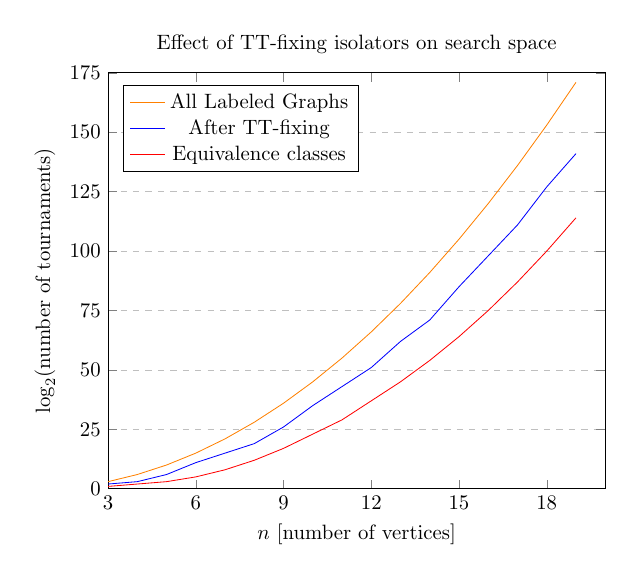
\begin{tikzpicture}[scale=0.75]
\begin{axis}[
    title={Effect of TT-fixing isolators on search space},
    xlabel={$n$ [number of vertices]},
    ylabel={$\log_2$(number of tournaments)},
    xmin=3, xmax=20,
    ymin=0, ymax=175,
    xtick={3,6,9,12,15,18},
    ytick={0,25,50,75,100,125,150, 175},
    legend pos=north west,
    ymajorgrids=true,
    grid style=dashed,
]

\addplot[
    color=orange,
    ]
    coordinates {
(3,3)(4,6)(5,10)(6,15)(7,21)(8,28)(9,36)(10,45)(11,55)(12,66)(13,78)(14,91)(15,105)(16,120)(17,136)(18,153)(19,171)
    };
    \addlegendentry{All Labeled Graphs}

\addplot[
    color=blue,
    ]
    coordinates {
    (3,2)(4,3)(5,6)(6,11)(7,15)(8,19)(9,26)(10,35)(11,43)(12,51)(13,62)(14,71)(15,85)(16,98)(17,111)(18,127)(19,141)
    };
    \addlegendentry{After TT-fixing}
    
\addplot[
    color=red,
    ]
    coordinates {
(3,1)(4,2)(5,3)(6,5)(7,8)(8,12)(9,17)(10,23)(11,29)(12,37)(13,45)(14,54)(15,64)(16,75)(17,87)(18,100)(19,114)
    };
    \addlegendentry{Equivalence classes}
    
\end{axis}
\end{tikzpicture}
\caption{A depiction of the search space reduction provided by TT-fixing using best-known Ramsey number bounds up to $n=18$ in $\log_2$ space.  }
\label{isosearchspace}
\end{figure}

\subsection{Practical vs Theoretical TT-fixing units}
We first note a useful recurrence relation on tournament Ramsey numbers: $R(k) \leq 2R(k-1)$. 
\begin{proof}
Consider an arbitrary vertex $v$ in an arbitrary tournament $G$ on $2R(k-1)$ vertices. $v$ must have either an out-degree or an in-degree of at least $R(k-1)$. In either case, consider the subset of at least $R(k-1)$ vertices pointed to/at by $v$. This subset must contain some $TT_{k-1}$ as a subgraph by definition of $R(k-1)$. However, $v$ points to or at all vertices in this $TT_{k-1}$, which demonstrates that a $TT_k$ comprised of the $TT_{k-1}$ vertices and $v$ exists in $G$. 
\end{proof}

In Figure \ref{pracunits} the bottom two lines depict the strict lower bound used in the $n\log n$ units proof (blue), as well as the actual number of units TT-fixing would provide if we only used the $R(k) \leq 2^{k-1}$ bound from the proof (red). Above that (orange) is the number of units TT-fixing provides given the best currently known Ramsey number bounds.  The best known bound on $R(7)$ is $34 \leq R(7) \leq 47$ \cite{directedramsey}, so the black line describes the best case for how many unit clauses TT-fixing could provide if $R(7) = 34$ was proven. The recurrence relation $R(k) \le 2R(k-1)$ is what allows even improvements to small Ramsey number bounds to impact the efficacy of TT-fixing for large $n$. %Figure \ref{lowerboundlarge} provides visual evidence of the tightness of the lower bound used in the proof. For all $n$ in the interval $[2,1e5)$ the maximum deviation of the two functions was 48, while the average deviation was $\approx 30.1$.

In Figure \ref{isosearchspace}, the top (orange) line is the total number of graphs a SAT solver must search in a tournament existence problem in the absence of an isolator.  The bottom (red) line is the number of unlabeled tournaments on $n$ vertices; this is the minimum number of graphs that any brute-force solver must search to solve a tournament existence problem. This data was taken from OEIS sequence A000568 \cite{ref_oeis}, which  limits the size of $n$ for which we can make this comparison to $n=19$. The middle (blue) line shows how many graphs are admitted by an isolator created by TT-fixing with the best known bounds on tournament Ramsey numbers. As $n$ grows large, the gap between the bottom two lines should grow small relative to the gap between the top two lines as per the $n \log n$ units upper bound proof.


\subsection{Undirected Isolators: Clique-fixing}
%\textbf{I cleaned this up a bit, is the description more understandable now or do you still think I should go with the cyclic approach to the clauses?}
As mentioned earlier, undirected isolators cannot have unit clauses. Therefore, undirected isolators cannot directly benefit from units via TT-fixing. However, a crossover result for undirected graphs does exist for binary clauses that uses the same ideas as TT-fixing; we term this process \emph{clique-fixing}. Undirected Ramsey number guarantee the existence of a red or blue colored $k$-clique for graphs with more than $R_u(k)$ vertices ($R_u$ used here for undirected Ramsey numbers). Clique-fixing uses the same iterative process as TT-fixing, but replaces the generation of units for $TT_k$ with the following clauses:

$\{r \lor e, \lnot r \lor \lnot e | e \in \mathit{Edges}(K_k)\}$
%$\{r \lor \mathit{idx}(b,c)  | (b, c) \in [1..k]\times[1..k] \text{ s.t. } b < c\}$

%$\{\lnot r \lor \lnot \mathit{idx}(b,c)  | (b, c) \in [1..k]\times[1..k] \text{ s.t. } b < c\}$

where $r$ is an auxiliary variable representing the concept ``the $k$-clique is red'' and $\mathit{Edges}(K_k)$ is the set of edge literals for the complete graph on $k$ vertices. We note that these clauses are ``almost'' units in the sense that after a solver makes a decision about whether to set $r$ to true or false, an entire $k(k-1)/2$ edges are set by unit propagation. Each step of clique-fixing therefore loses a single unit clause worth of search space reduction when compared to TT-fixing. Although not the focus of this work, it is plausible that a similar asymptotic optimality analysis could be done for clique-fixing given this small discrepancy. However, it is notable that undirected Ramsey numbers (necessary for clique-fixing) empirically grow much faster than tournament Ramsey numbers despite equal theoretical worst-case scaling, which implies that clique-fixing may not be as practically useful as TT-fixing.


%\begin{figure}
%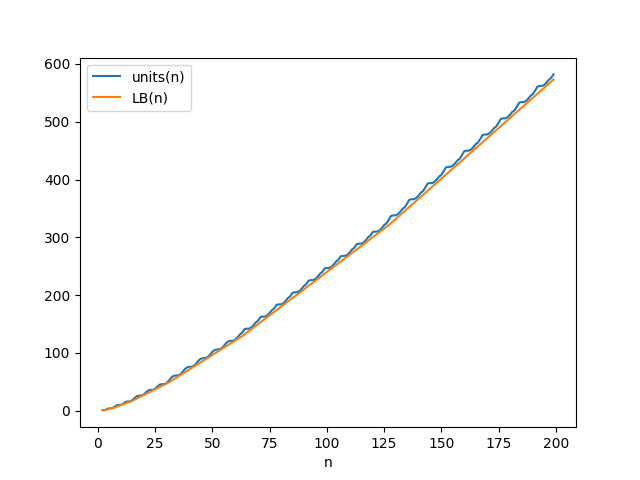
\includegraphics[width=0.6\textwidth]{nlogn_200.png}
%\caption{Comparison of $units(n)$ and the proven lower bound denoted as $LB(n)$} \label{nlogn_200}
%\end{figure}

%\begin{figure}
%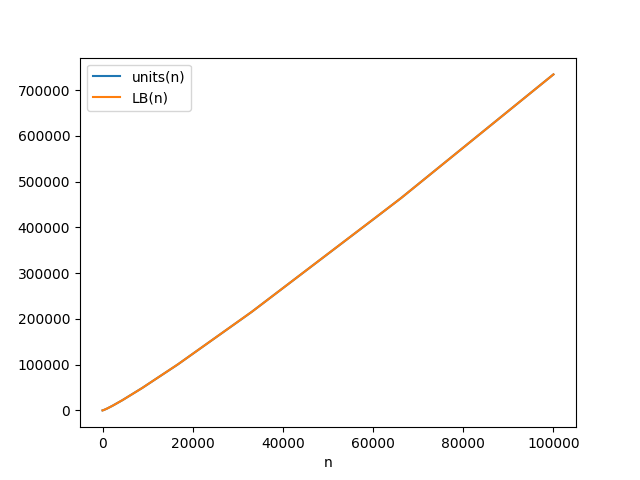
\includegraphics[width=0.4\textwidth]{nlogn_huge.png}
%\caption{Comparison of $units(n)$ and the proven lower bound denoted as $LB(n)$ for large $n$} \label{nlogn_huge}
%\end{figure}







\section{Perfect, Optimal Isolator SAT encoding}

Unit-based techniques scale to arbitrary $n$, and TT-fixing is ``asymptotically perfect'' in the sense that for large tournaments, no isolator generation technique can provide more than a non-constant factor of search space reduction over TT-fixing. However, no known perfect isolators for $n>4$ consist solely of unit clauses. Additionally, it can be practically useful to have an \emph{optimal} perfect isolator for small tournaments to allow searching via SAT solver for only non-isomorphic (sub-)graphs as efficiently as possible. The practical utility of compact perfect isolators is demonstrated in our own experiments in the later ``Tournament Ramsey Graphs'' section. In the following sections, we describe our technique for creating perfect, optimal isolators for $n \le 6$.

\subsection{Basic SAT encoding}

We re-implemented and modified the perfect isolator encoding for undirected graphs \cite{ref_heule} to be used for tournaments. Formally, we encoded the question ``Is there a set of $k$ clauses $C_1, C_2, ... C_k$ that is a perfect isolator for $n$-vertex tournaments.'' Decoding a solution to this formula allowed us to produce an $n$-vertex isolator with $k$ clauses. %This first section will explain the encoding of the simpler problem: ``Is there a set of $k$ clauses $C_1, C_2, ... C_k$ whose union is a perfect isolator for $n$-vertex tournaments,'' which will be modified to the final problem definition in following sections.

For the $i$th isolator clause $C_i$ and arc literal $l$, we defined the variable $\mathit{In}(C_i, l)$ to represent ``$l$ is in $C_i$''. Then, for each tournament $G$ on $n$ vertices, we define variables $\mathit{Excludes}(G,C_i)$ for $1 \le i \le k$ to mean ``clause $C_i$ does not admit $G$.'' This specification is implemented as follows with a Tseitin encoding \cite{ref_tseitin} to handle the equality and conjunctions:

\begin{equation}
\mathit{Excludes}(G,C_i) \leftrightarrow \bigwedge\limits_{l \in A_G}\lnot \mathit{In}(C_i, l).
\end{equation}

\noindent Here $A_G$ is the set of arc literals corresponding to the arcs present in graph $G$. We also define the variable $\mathit{Canon}(G)$ for all graphs $G$, meaning ``Graph $G$ is the canonical representative of its isomorphism class $I_G$.'' We implement this as follows (again using Tseitin):

\begin{equation}
    \mathit{Canon}(G) \leftrightarrow \bigwedge\limits_{i=1}^k \lnot \mathit{Excludes}(G,C_i).
\end{equation}

Finally, for each isomorphism class $I$, we add the following clauses representing ``exactly one graph in $I$ is canonical'' to the formula for each isomorphism class $I$:

\begin{equation}
 %\mathit{AMO}(E_1) \land \bigvee\limits_{C \in E_1} C.
 \mathit{ExactlyOne}(\{\mathit{Canon}(G) | G \in I\})
 \label{eq:perfisoform}
\end{equation}
\noindent Here $\mathit{ExactlyOne}$ is implemented with an At Most One operation via Sinz encoding \cite{ref_sinz} and an At Least One via disjunction. Therefore, a satisfying assignment to this formula corresponds to a perfect isolator on $k$ clauses. If the formula is unsatisfiable for $k$ and satisfiable for $k+1$, then the perfect isolator with $k+1$ clauses is optimal for the $n$ in question.


\subsection{Symmetry Breaking}

One symmetry in the above encoding is the order of the isolator clauses, as reordering clauses of an expression in CNF does not affect its satisfying assignments.  To break this symmetry, we added clauses that ensured a lexicographic ordering of the clauses in the resulting isolator.  For every adjacent pair of clauses $C_i$ and $C_{i+1}$, we fixed some ordering of every literal that may appear in them $l_1, l_2, \dots, l_n$, and then created variables $e_0, e_1, \dots, e_n$ where $e_j$ represents that clauses $C_i$ and $C_{i+1}$ are equivalent when considering only the first $j$ literals.  $e_0$ is always true, and to maintain the semantics of the other $e_j$ we added the clauses
$$e_j \leftrightarrow (e_{j-1} \land (\mathit{In}(C_i, l_j) \leftrightarrow \mathit{In}(C_{i+1}, l_j)))$$
via the Tseitin transformation for every $1 \le i < k$ and $1 \le j\le n$.  Then, we enforced a lexicographic ordering by requiring that for every $j$ such that $C_i$ and $C_{i+1}$ were equal up to $j$, that if clause $C_i$ contained $l_j$ then $C_{i+1}$ must also contain $l_j$.  Explicitly, we added the following requirement via the Tseitin transformation for every $1 \le i < k$ and $1 \le j\le n$:
$$e_{j-1} \land \mathit{In}(C_i, l_j) \implies \mathit{In}(C_{i+1}, l_j)$$
and furthermore we required that $e_n$ is false to ensure a strict ordering.  When searching for an isolator with $k$ clauses, this reduces the search space by a factor of $k!$ as only one of the $k!$ permutations of a given distinct set of clauses will be considered.

There is another symmetry in the vertex labeling.  For a given isolator, for each literal $l$ corresponding to arc index $I_{ab}$, we can change $l$ to correspond to arc index $I_{\pi(a),\pi(b)}$ where $\pi$ is a permutation of vertex labels. The resulting isolator accepts the same graphs that the original did, but under vertex permutation $\pi$.  To break this symmetry, note that any tournament isolator must admit exactly one transitive tournament.  So, we choose to admit only the canonical transitive graph with edges of the form $(v_i, v_j), i < j$.  Note that because every edge in this graph goes from a lower numbered vertex to a higher numbered vertex, the corresponding literals in our encoding are all positive.  As such, we know that for any isolator, there is a permuted isolator such that every clause has at least one positive literal in each clause.  We may add this to our encoding by requiring for all clauses $C$
$$\bigvee_{l \in A_p} \mathit{In}(C, l)$$
with $A_p$ being the set of all positive literals.    When trying to find an isolator for $n$ vertices, this reduces the search space by a factor of $n!$ since the solver is guaranteed to only consider isolators for which the canonical transitive graph is the one described above.

\subsection{Encoding Unit Propagation}

Under the encoding described above, our solver finds isolators with many large clauses. However, by applying unit propagation it was often possible to reduce clause sizes. This indicated that not only was the solver generating solutions that needed postprocessing, but candidate isolators that were equivalent under unit propagation were being considered multiple times --- a sort of symmetry in this problem.  To resolve this, we added variables $\mathit{Unit}(l)$ representing ``literal $l$ is a unit clause.'' We then required that the isolator be already unit-propagated with respect to these literals by adding the requirement
$$\lnot \mathit{In}(C, l) \lor \lnot \mathit{Unit}(l)$$
for all clauses $C$ and literals $l$. We also had to account for these units excluding graphs in the $\mathit{Canon}$ clauses, which were updated to
$$\mathit{Canon}(G) \leftrightarrow \bigwedge\limits_{i=1}^k \lnot \mathit{Excludes}(G,C_i) \land \bigvee\limits_{l \in A_G}\lnot \mathit{Unit}(\lnot l)$$


Finally, we considered whether to count these special unit literals towards the clause count in determining isolator optimality. As mentioned in the preliminaries, we chose not to do so. When an isolator with units is used in a SAT solver, the units will be instantly eliminated through unit propagation and thus will reduce the complexity of the resulting problem.  Therefore, we consider an optimal isolator to not just have the minimal number of clauses, but the minimal number of non-unit clauses.  Since units cannot exist in undirected graph isolators (because an undirected graph isolator must admit both the complete and empty graph), this definition of optimality is consistent with the prior work on the undirected case \cite{ref_heule}. Note that we only needed to consider positive unit literals as per the vertex-labeling symmetry breaking, which drastically reduced the search space.

%We decided to not count units towards the clause count for use in determining optimality because of this.  This is not only a more useful definition, but results in a less complex encoding as we do not need to count objects of two different types, and we do not need to ensure that the non-unit clauses are actually not units.  The last is due to the fact that since units are `free' in our setup and non-units are costly, a solution to our encoding that uses a non-unit clause position to encode a unit will have wasted that position, and a solution that holds for fewer allowed non-units will simply move that clause to a unit literal position.

%Note that using the direction symmetry breaking above, we only need to consider positive unit literals, which drastically reduces the search space in this step.


%While constructing smaller isolators using the techniques above, we opted to manually inspect our results and see what patterns they shared.  Specifically, in the isolators up through 6 vertices there were some very noticable patterns in the unit clauses they contained, at least after permuting the isolators' vertices to line them up with each other.  The easiest structure to notice was that all of these isolators contained an $n-1$--length path, or a directed path that touches every vertex exactly once.  In graph theory literature, this is known as a Hamiltonian path.

%As it turns out this pattern of units admits a proof, and so without worry we can include it in the basis for any isolator.

%\newtheorem{
%All tournament graphs admit a Hamiltonian path.}{}


%\begin{proof}
%Proceed by induction.  The statement is trivial for 1- and 2- vertex tournaments, since in the former the empty path is Hamiltonian and in the latter the sole edge is the path.  Now, given an $m$-length path in a tournament for $2 \le m < n-1$, argue that an $m+1$-length path exists.

%Label the vertices on the given path by $1$ through $m+1$, and since $m+1 < n$ there exists some other vertex $a$.  If there is an edge from $a$ to $1$ or $m+1$ to $a$, then we can trivially extend the path to include $a$, so take the other case where there is an edge from $1$ to $a$ and an edge from $a$ to $m+1$.  Consider the smallest $1 \le i \le m+1$ such that there is an edge from $a$ to $i$.  Clearly $i > 1$ as there is an edge from $1$ to $a$, and clearly $i$ is well-defined since the set of $i$ where there is an edge from $a$ to $i$ is nonempty as it contains $m+1$.  Then, we have that $i-1 \ge 1$, and furthermore there is no edge from $a$ to $i-1$, so there is an edge from $i-1$ to $a$.  Therefore, we can take $i-2$ steps on the original path from vertex $1$ to vertex $i-1$, one step from $i-1$ to $a$, one step from $a$ to $i$, and $m+1-i$ steps on the original path from vertex $i$ to vertex $m+1$.  This new path has length $(i-2) + (1) + (1) + (m+1-i) = m+1$, completing the induction step and thus the proof.  $\square$
%\end{proof}

%It is worth noting that we do not have a proof that fixing a Hamiltonian path in an isolator is optimal.  However, getting a large set of units for free is extremely helpful, especially since our map-file approach does not need to consider graphs that are made impossible by a basis set of units. Including these units reduces the map file size and generation time by a factor of $2^{n-1}$, which makes map file-based approaches still viable for up to $n = 8$, and the risk of it being suboptimal (especially by a large factor) seems intuitively very low.






\section{Additional Isolator Generation Techniques}

The following sections describe several miscellaneous techniques, ranging from practical ways to gain slight improvements on prior techniques to possible directions for future research.

\subsection{Incremental Isolators}
Prior work has already shown that any isolator for $n$-vertex tournaments is also an isolator for $n+k$-vertex tournaments for any positive $k$, and that combining an isolator on $m$ vertices with an isolator on $n$ vertices by applying each isolator to a disjoint subset of vertices creates a new isolator on $m+n$ vertices \cite{ref_incremental}. Therefore, it is possible to construct perfect isolators for $n+k$-vertex tournaments by adding clauses to any isolator for $n$-vertex tournaments. In particular, our SAT encoding pipeline had the option to ignore graphs that are not admitted by a given set of units. Including the maximal set of units from an $n$-vertex isolator when generating an encoding for $n+1$-vertex isolators reduces the number of tournaments to generate $\mathit{Canon}$ clauses for by a factor of at least $2^{n}$ because each isolator has at least the units corresponding to a Hamiltonian path. It is worth noting that we do not have any proofs that any of our non-perfect or non-optimal isolators can be extended to an \textit{optimal} isolator, even when the isolator being extended from is comprised of only unit clauses.  However, extending an isolator from an initial set of units can make searching for compact isolators much more efficient. 

%We further note that it is always possible to combine an isolator on $m$ vertices with an isolator on $n$ vertices to create a new isolator on $m+n$ vertices. The method for doing so involves applying each isolator to a disjoint subset of vertices. More formally, given two injective functions $f_m: [1,m] \rightarrow [1,m+n], f_n: [1,n] \rightarrow [1,m+n]$ s.t the ranges of $f_m$ and $f_n$ are disjoint, each literal representing some arc $(a,b)$ in the $m$-vertex isolator gets transformed to the literal representing arc $(f_m(a), f_m(b))$, and likewise with $f_n$ for the $n$-vertex isolator. The resulting isolator is valid by the following proof.

%\begin{proof}
%Consider an arbitrary $m+n$-vertex tournament $g_{mn}$; it contains disjoint subtournaments $g_m,g_n$ on $m$ and $n$ vertices selected by considering the ranges of $f_m, f_n$ as defined above. $g_m$ and $g_n$ are admitted by $m$ and $n$ vertex isolators respectively under some permutations $\pi_m,\pi_n$ on the ranges of $f_m, f_n$. Composing $\pi_m$ and $\pi_n$ and applying the resulting permutation to $g_{mn}$ produces a graph isomorphic to $g_{mn}$ admitted by the conjunction of the two isolators, proving that every equivalence class has at least one member admitted by said union.
%\end{proof}

The technique of combining disjoint isolators is practically useful for creating compact isolators for large $n$. Although TT-fixing guarantees asymptotic optimality, when the procedure reaches the point of generating units for $k=8$ or fewer remaining vertices, more units can be added by using the units from a known compact isolator for $k$ vertices. For example, TT-fixing will generate 9 units when processing 8-vertex (sub)tournaments, while our isolator for $n=8$ contains 11 units. 

%\textbf{figure describing the composite process TBD}

%One way to view the inclusion of a Hamiltonian path in our problem definition for each $n$ is that the unit clauses used to encode the isolator search problem for $n+1$ vertices build off the set of isolators used in the $n$ case (by simply adding the positive unit corresponding to the arc $(n, n+1)$). We further generalize this idea by showing that it is always possible to extend an isolator for $n$-vertex tournaments (and, incidentally, undirected graphs) to an isolator on $n+1$ vertices. Let $P_n$ be an isolator, defined here as a predicate on $n$-vertex tournaments that admits at least one tournament from each isomorphism class. Further, $[G]_n$ for a tournament $G$ on $n+1$ vertices refers to the tournament formed by removing the $n+1$th vertex of $G$.

%\newtheorem{
% For any $P_n$, a predicate $P_{n+1}$ that admits the $n+1$-vertex $G$ iff $P_n([G]_n)$ holds is an isolator on $n+1$-vertex tournaments.}{}

%\begin{proof}
%Consider any canonical set containing representatives $R$ from each isomorphism class of $n+1$-vertex tournaments. For each $R$, $[R]_n$ is an $n$-vertex tournament and therefore a member of one of the isomorphism classes on $n$-vertex tournaments. By definition, the arbitrary given $P_n$ admits some $r$ such that $r \simeq [R]_n$. Any two isomorphic $n$-vertex tournaments are related by some vertex permutation $v_n$, where we define $v_n(r)$ for a tournament $r$ to be the tournament constructed by the application of $v_n$ to each vertex of $r$. Therefore we have $v_n(r) = [R]_n$ for some $v_n$.

%This $v_n$ can be extended to tournaments on $n+1$ vertices via $v_{n+1}(x) = v_n(x)$ when vertex $x$ is not vertex $n+1$, and $v_{n+1}(x) = n+1$ otherwise.  Applying each $v_{n+1}^{-1}$ (the inverse permutation of $v_{n+1}$) to its corresponding $R$ yields a new canonical set $S$ for $n+1$-vertex tournaments because tournament isomorphism classes are closed under vertex permutation. We claim that $P_{n+1}$ admits all members of $S$, making it an isolator. To check this, note that each new canonical representative is of the form $v_{n+1}^{-1}(R)$ for some $R$. By definition of $P_{n+1}$, we must confirm that $P_n([v_{n+1}^{-1}(R)]_n)$ holds. However, $[v_{n+1}^{-1}(R)]_n = v_n^{-1}([R]_n) = r$, and $P_n(r)$ holds by the definition of $r$, completing the proof. $\square$
%\end{proof}

%The idea for incremental isolators and its following proof fell out of the observation that the optimal isolator for $n=5$ had striking similarities to the optimal isolator for $n=4$. In fact, it is possible to build directly off the entire $n=4$ isolator when constructing an optimal isolator for $n=5$. However, in general a perfect $n+1$-vertex isolator constructed incrementally from an optimal, perfect $n$-vertex isolator is not optimal, with a counterexample appearing at $n=6$. We note that it is also possible to build $n+1$-vertex incremental isolators from any subset of clauses from an $n$-vertex isolator. The most natural choice of subset when pursuing optimal isolators would be the unit clauses, because it kills the most non-canonical graphs. We were not able to prove that isolators built from incremental units are optimal or suboptimal in general, but it produces optimal isolators in practice up to $n=6$. The incremental units approach is a generalization to the approach of fixing the Hamiltonian path units, and allows a further reduction of the space of considered isolators.

\subsection{Probing}
In addition to the SAT encoding approach to isolator generation, we also generated isolators using a method from prior work called ``random probes''  \cite{ref_heule}. On a high level, this approach starts with an empty set of clauses and adds randomly generated clauses that preserve at least one member of each equivalence class until the isolator is perfect.  There were only two non-superficial changes needed to adapt the prior work on random probes for undirected graphs to the directed case; allowing unit clauses and allowing clauses with only positive literals. While not guaranteed to generate optimal isolators, the strength of this approach is the relative speed with which isolators are generated. This approach also benefited in efficiency from the technique of disallowing clauses with all negative literals and extending isolators from the unit clauses of smaller isolators.

%\subsection{Canonical set techniques}
%One major criticism of our approaches for producing \textit{perfect} isolators is that they do not scale to $n>9$. Already at n=9 there are $2^{36}$ labeled tournaments on $9$ vertices; this number can be reduced by enforcing all 13 known possible unit clauses during the generation of the CNF file, but the CNF produced by our SAT-based method is not solvable in several days, and probes for $n=8$ take $\sim 2$ days compared to several seconds for $n=7$. As such, we also experimented with a canonical-set-based approach that scales with the number of equivalence classes. 

%The canonical-set-based approach uses the well-known idea that one way to create an isolator is to generate one canonical representative for each equivalence class, then construct a formula that admits exactly those graphs \cite{ref_canon_set}. Our approach differed slightly from \cite{ref_canon_set}, as instead of using lexicographic ordering constraints from a carefully constructed ``canonizing set'' on the graph's adjacency matrix, we express any given set of canonical representatives in disjunctive normal form (DNF), then convert the DNF to CNF using Bica \cite{ref_bica}. Because this approach may lead to much larger isolators than the optimal ones, we first used the canonical sets induced by our optimal isolators as proofs of concept. As seen in the ``optimal'' column of  table \ref{tab:canon_set}, the resulting CNFs were equal in number of clauses to our optimal isolators up to n=6 (our isolators for n=7 and above are not optimal, and thus were not considered). Next, we tried the naive approach of using the canonical set produced by the NAUTY \cite{ref_nauty} program. The size of the isolators generated was very suboptimal, as the canonical form used by NAUTY does not enforce common edges (column ``arbitrary'' in table \ref{tab:canon_set} below).

%A more promising approach involves modifying a given arbitrary canonical set to have certain properties. Given a canonical set, we detect a Hamiltonian path in each member of the set via an algorithm modeled on the proof of Hamiltonian path existence, then permute each member of the canonical set to have the path $(v_1,v_2),(v_2,v_3),... (v_{n-1},v_n)$. The motivation of this procedure is to cause the canonical set members to have more edges in common, which will lead to more unit clauses in the final CNF. These experiments gave better results than the naive approach, but did not succeed in matching the true optimal isolator length (see ``heuristic'' column of  table \ref{tab:canon_set}). A possible direction for future work is the development of heuristics for permuting canonical set representatives to produce canonical sets admitting short isolators.

%\begin{table}[ht]
%    \centering
%        \caption{Isolators found with canonical set techniques}
%    \begin{tabular}{c|c|c|c|c}
%        Vertices & Isomorphism classes & optimal & heuristic & arbitrary  \\ \hline
%        4&4&4&6&8\\
%        5&12&8&16&24\\ 
%        6&56&14&42&62\\ 
%        %7&456&n/a&47\\ 
%    \end{tabular}
%
%    \label{tab:canon_set}
%\end{table}

\section{Results}

Our experimental results include the sizes of known perfect isolators for small $n$, as well as experiments showing the practical utility of small $n=6,7$ perfect isolators for solving a tournament existence problem.

\subsection{Experimental Setup}
Our SAT-based approach to generating isolators rely on the creation of ``map'' files: text files associating each tournament of size $n$ with a label representing that graph's isomorphism class. In order to generate a map file for tournaments on $n$ vertices, we began by enumerating all $2^{n(n-1)/2}$ graphs of size $n$. We converted each graph into an adjacency matrix and then into the ``.d6'' format specified in the NAUTY handbook, then fed the resulting graphs into the labelg script bundled with the NAUTY tool for graph isomorphisms \cite{ref_nauty}. labelg produced a file where each graph was converted to the canonical form used by nauty. We gave each canonical form a unique label and outputted the arc (directed edge) indices of each original graph alongside its canonical form. 
%When outputting graphs for the map file we simply exclude all negative arc indices to reduce file size, as the negative edges can be inferred with knowledge of $n$ because tournaments are complete graphs. An example map file line for $n=5$ tournaments is:
%\begin{verbatim}11    2 5 7 0\end{verbatim}
%The first number in the line ($11$) is the arbitrary label given to the isomorphism class of the graph described by the rest of the line. The remaining non-zero numbers describe all lexicographically increasing arcs present in the graph. In particular, Arc index $2$ represents the arc $(1,3)$, $5$ represents $(2,4)$, and $7$ represents $(1,5)$. So, all other vertex pairs in this tournament have arcs in lexicographically decreasing order, i.e. vertex $5$ is connected to vertices $4$ and $3$ by the arcs $(5,4)$, $(5,3)$. Each line is terminated with a 0, following a convention from CNF.


\subsection{Small Optimal Isolators}

Our SAT encoding allowed us to compute optimal isolators up to $n=6$. The SAT solver CaDiCaL \cite{cadical} solves the two instances required to prove optimality ($k=6,7$ non-unit clauses) within 24 hours. Figures \ref{iso4} and \ref{fig2} graphically display optimal, perfect isolators for $n=4,5$ by displaying a graph from each isomorphism class. Figure \ref{fig3} presents the same image for one of the 56 isomorphism classes for $n=6$. Most of the structure of these isolators can be seen from their unit clauses, which are depicted via red edges in the figures. 

%For $n=4,5$ we also computed the number of different perfect optimal isolators up to isomorphism, where we define two isolators to be isomorphic if they are equivalent under some vertex permutation. There is only a single perfect optimal isolator for $n=4$, while there are 5 different (perfect optimal) isolators for $n=5$. Interestingly, each of the 5 can be expressed such that they have the same 6 unit clauses, and differ only in the 2 non-unit clauses present in optimal $n=5$ isolators.

%\begin{figure}
%\centering
%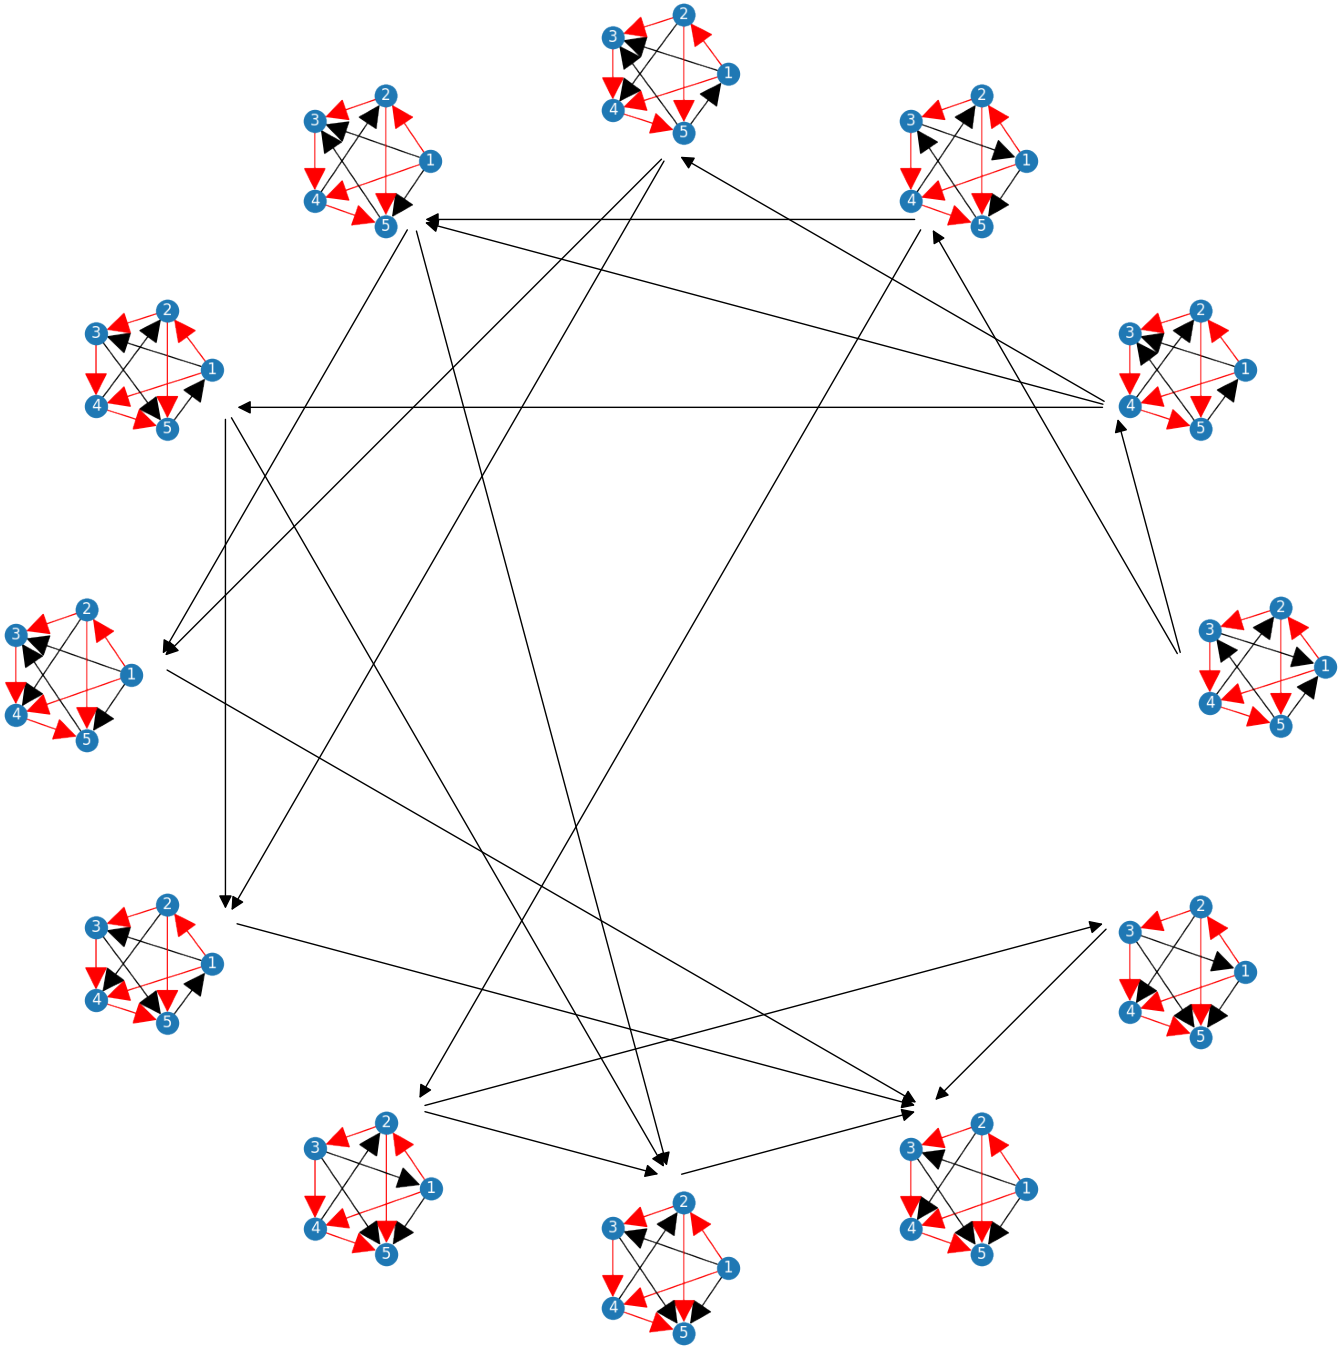
\includegraphics[width=0.4\textwidth]{ramsey_5_flowchart.png}
%\caption{Flowchart showing one-off relationships between n=5 equivalence classes} \label{flowchart}
%\end{figure}

\begin{figure}
\centering
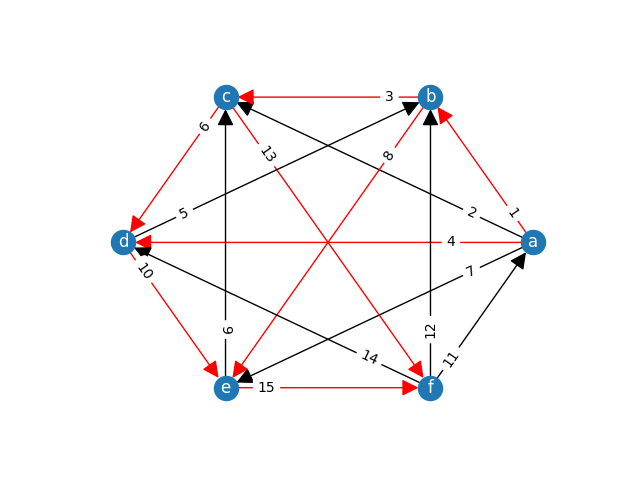
\includegraphics[width=0.4\textwidth]{iso6.png}
\caption{One of the 56 Isomorphism class representatives admitted by a particular isolator for 6-vertex tournaments. Red edges are edges fixed by unit clauses of the isolator.} \label{fig3}
\end{figure}
%mention the number of unique isolators up to isomorphism

%\subsection{Larger Isolators}

 For $n = 7$, solving the SAT instance directly became clearly infeasible (taking several days without any signs of progress). However, random probing allowed us to find a perfect isolator. Each probe ran in around 10 seconds when restricted to force a positive literal in each clause with the map file reduced by the unit clauses from $n=6$.  Table \ref{tab:smallest_isolators_found} describes the best (fewest non-unit clauses) isolator found for $1 \le n \le 7$. Several thousand probes were required to find our best known isolator for $n=7$.

\begin{table}[ht]
    \centering
        \caption{Shortest isolators found for $n\le 7$}
    \begin{tabular}{c|c|c|c}
        Vertices & Isomorphism classes &Best units & Best non-units  \\ \hline
        1&1&0&0\\ 
        2&1&1&0\\ 
        3&2&2&0\\ 
        4&4&4&0\\
        5&12&6&2\\ 
        6&56&8&6\\ 
        7&456&9&47\\ 
    \end{tabular}

    \label{tab:smallest_isolators_found}
\end{table}

\begin{figure}
\centering
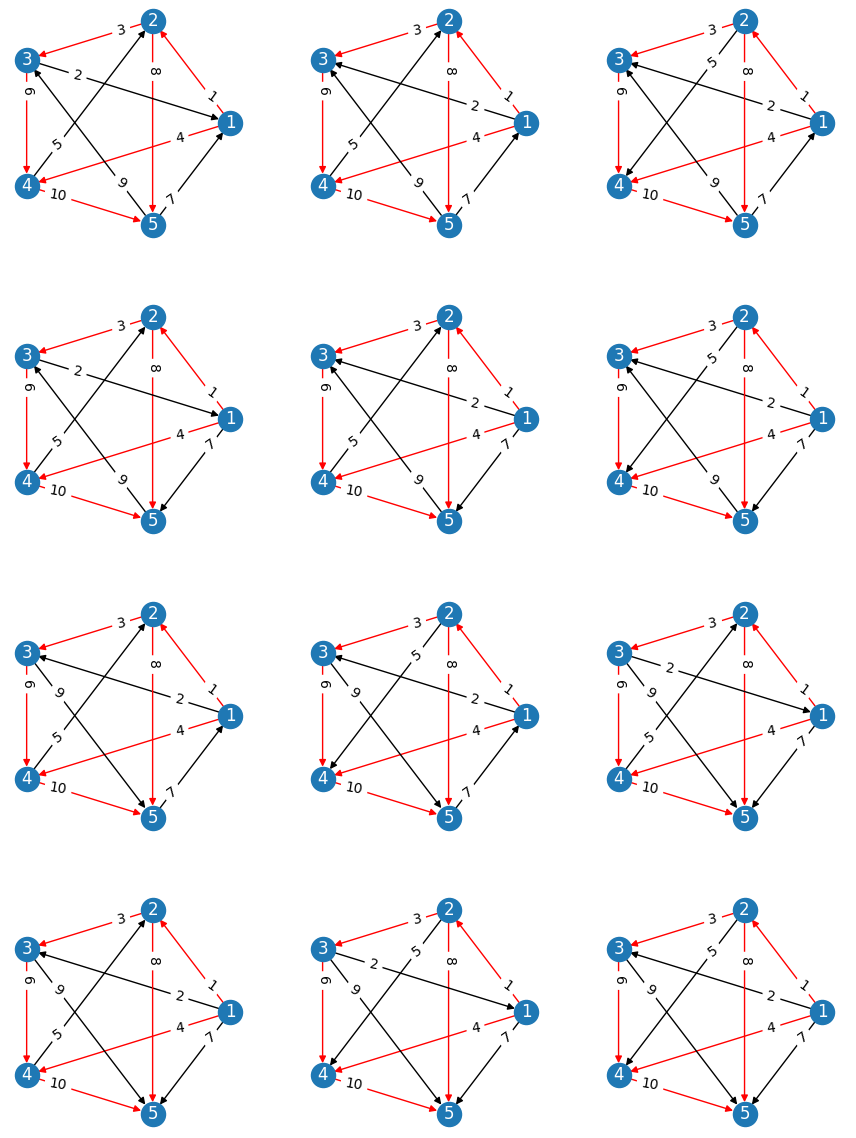
\includegraphics[width=0.5\textwidth]{iso_5.png}
\caption{All isomorphism class representatives admitted by a particular isolator for 5-vertex tournaments. Red edges are edges fixed by unit clauses of the isolator. The two non-unit clauses in the isolator are $2 \lor -5 \lor 9$ and $2 \lor 7 \lor -9$.} \label{fig2}
\end{figure}

\subsection{Tournament Ramsey Graphs}

The known Ramsey tournaments numbers are $R(2) = 2$, $R(3) = 4$, $R(4) = 8$, $R(5) = 14$, and $R(6) = 28$~\cite{}. Note that in most cases, the next number is two times it predecessor. Recently, 
the lower and upper bounds for $R(7)$ have been improved from $32 \leq R(7) \leq 54$ to $34 \leq R(7) \leq 47$~\cite{}. The improved lower bound is due to dozens of $TT_7$-free tournament on 33-vertices found using SAT. 

McKay~\cite{} extended this set of 33-vertex $TT_7$-free tournaments to 5303 using the following method: generate all 29-vertex sub-tournaments of known 33-vertex $TT_7$-free tournaments and extend them in all possible ways to 33-vertex $TT_7$-free tournaments. Repeat this procedure until no new 33-vertex $TT_7$-free tournaments are found. Also note that if a tournament has no $TT_k$, then its complement (reversing all arcs) also doesn't. This can be used to find additional $TT_k$-free graphs as well. 

Looking for neighbors and complement graphs is a well-known technique to compute more graphs with a certain property. McKay and Radziszowski used it to compute all known 42-vertex graphs that have no clique of size 5 nor a co-clique of size 5~\cite{}. They conjecture that this method generated all possible graphs of this type. 

If for some $n$ there exists a $k$ with a unique $TT_k$-free tournament on $n$ vertices, then that graph is known as ST$n$. We studied the 5303 33-vertex $TT_7$-free tournaments and
found that all of them have ST26 as a subtournament. Moreover, 4952 of them have ST27 as a subtournament. 

%Let $TR(n, k)$ be the set of unlabeled (equivalently, labeled but up to isomorphism) tournaments on $n$ vertices that contain no $TT_k$ as a subgraph. The tournament Ramsey problem asks for the smallest $n$ such that $|TR(n, k)| = 0$ given some fixed $k$. To improve a tournament Ramsey number lower bound, it suffices to find a tournament without a $TT_k$ larger than any known tournament without a $TT_k$. One method for doing so is attempting to extend one of the largest known tournaments without a $TT_k$, because any larger tournament with a $TT_k$ necessarily has at least one smaller such tournament as a subgraph (up to isomorphism).
%
%Therefore, one direct method for incremental progress towards improving tournament Ramsey number bounds is to expand the known portion of $TR(n,k)$ for the maximal known $n$ for some fixed $k$. In particular, we sought to use our isolator techniques in conjunction with the methods of earlier work on tournament Ramsey numbers \cite{directedramsey} to find more members of $TR(33,7)$. All isomorphism checking and automorphism generation referred to below was done with the NAUTY \cite{ref_nauty} tool.
%
%For certain $n,k$ it is the case that $|TR(n,k)| = 1$. In such cases, the graph ST$n$ refers to the single member of $TR(n,k)$. For example, ST$25$, ST$26$, and ST$27$ are the only tournaments on $25,26,27$ vertices respectively without a $TT_6$ \cite{ref_early_tournament_ramsey}. Out of the 5303 members of $TR(33,7)$ found prior to this work \cite{directedramsey}, all contained ST$25$ and ST$26$ as a subgraph, while all but 352 members contained ST$27$. While every tournament in the known portion of $TR(33,7)$ contained exactly 0 or 1 subgraph isomorphic to ST$27$, each tournament had between $2$ and $39$ (inclusive) subgraphs isomorphic to ST$26$, with the vast majority having 27 due the existence of ST$27$ in the graph (removing any vertex from ST$27$ yields ST$26$).

We explored whether the suite of 5303 was complete or whether there are any other 33-vertex $TT_7$-free tournaments.
 Our main experimental setup involved finding new members containing ST$26$ but not ST$27$ by solving a CNF formula with a SAT solver, which uses our isolator on 7 vertices. The formula can be described as the union of the following sets of clauses:
 
 \begin{enumerate}
 \item ${26 \choose 2} = 325$ unit clauses requiring that ST26 be present in vertices $v_1$ through $v_{26}$
 \item The perfect isolator for $n=7$ on the seven remaining vertices $v_{27}$ through $v_{33}$
 \item A clause blocking each of the 5303 known solutions for each vertex permutation that caused the solution to have ST$26$ in vertices $v_1$ through $v_{26}$ and a graph admitted by the $n=7$ isolator in vertices $v_{27}$ through $v_{33}$
 \item clauses enforcing the ``no $TT_7$'' condition from \cite{directedramsey}
 \end{enumerate}

While this formula does not disallow all ST$27$s (i.e. a solution might include an extension from ST$26$ that was not present in the original solution set), it disallows all currently known extensions, including the most common by far $1$-vertex extension from ST$26$ to ST$27$. Additionally, the $n=7$ perfect isolator plays a crucial role for finding new solutions in that without it, the SAT solver could find any tournament equivalent to one of the previously known 33-vertex $TT_7$-free tournaments  except for some non-automorphic permutation of the last 7 vertices (which would thus be isomorphic to the previously known solution). We claim that all solutions to our formula must be non-isomorphic to the original 5303 solutions. 

We ran 640 shuffled (clause permuted) versions of the above formula on 640 cores for 6 hours using Kissat. We found three different satisfying assignments. These three solutions represented  a single new 33-vertex $TT_7$-free tournament. This tournament is special as it is self-complementary: reversing all arcs result in an isomorphic graph. Only a small fraction of tournaments has this self-complementary property~\cite{}. Note that all ST$n$ graphs have this property by definition. After finding this new tournament, we updated the formula to include the blocking clauses for the new tournaments and its isomorphisms. Kissat did not produce further solutions when using 640 shuffled (clause permuted) version of the updated formula on 640 cores in a day, so it is possible that the formula is simply unsatisfiable. In conclusion, the formula we produced allows an efficient and effective way to find a new 33-vertex $TT_7$-free tournament. 
%\subsection{Maximal Unit Sets}
%probably not needed, not actually interesting either without a bunch of figures to show the sets

%\section{Future Work}

%\subsection{Limitations of Current Approach}

%imperfect but good isolators?
%\subsection{Removing the Map File}

%In our current setup, generation of the SAT problems involves mapping all possible tournament graphs to their isomorphism class.  Since this grows at a rate of $2^{O(n^2)}$, this becomes prohibitively large very quickly.  Even only considering graphs that satisfy a basis set of units, such as the Hamiltonian path or the prior isolator's units, these approaches quickly become infeasible as soon as $n = 9$.  By only generating the graphs that satisfy the previous isolator (and not just the units), this approach could potentially be extended for slightly longer, albeit at the cost of almost certainly suboptimal isolators.  A more clever encoding, or some way of encoding some of the ideas of graph isomorphism into the problem itself, could potentially drastically reduce the size of the problems and find isolators for much larger tournaments.

%\subsection{Isolator Applications}

%Graph existence problems, or problems that relate to whether a graph satisfying some conditions exist, are notoriously difficult to solve.  The Ramsey numbers, Conway's 99-graph problem, and many other problems can be phrased (or are most directly phrased) in this manner remain open problems in their fields even for relatively small instances.  For this reason computational approaches are tempting since they might be able resolve smaller instances of these problems, at least with an efficient enough algorithm.  Isolators provide a mechanism by which SAT solvers might be able to go fast enough to help in this area, since they drastically reduce the search space of possible graphs and leave only the non-redundant cases to check.

%The main motivation towards finding these tournament graph isolators is their potential uses in computing tighter bounds on tournament Ramsey numbers --- the directed analog of Ramsey numbers for tournaments.  The tournament Ramsey number at $n$ is defined to be the smallest $m$ such that all tournaments on $m$ vertices contain a transitive (cycle-free) subtournament of $n$ vertices.  SAT approaches have been taken with this problem before to tighten bounds on the directed Ramsey number $R(7)$ \cite{directedramsey}.  From this it seems very likely that directed isolators --- boosted by their simplicity / number of unit clauses in them --- should be able to be applicable on this problem and potentially tighten those bounds further.


%\section{Generating Optimal Perfect Isolators}

%%Symmetry breaking is often a key challenge in encoding search problems into SAT instances. \textbf{mention some particularly important problems using SB}.

%The goal of graph existence problems is to prove the existence of an unlabeled graph satisfying certain conditions. For example, one method for computing Ramsey numbers (a foundational problem in Ramsey theory) is by showing that there exists a graph with $n$ vertices that contains a clique or independent set of size $k$, but there does not exist such a graph with $n+1$ vertices. 

%Graph existence problems can often easily be encoded to SAT by disallowing all sets of edges that could cause a graph to not satisfy the desired property (i.e. for Ramsey numbers, disallow all possible size-$k$ cliques and independent sets). However, the SAT approach to graph existence problems tends to be outperformed by specialized tools \textbf{CITE}. 

%The underperformance of SAT on these types of problems is at least partially due to suboptimal encodings \textbf{CITE}. We observe that if a graph $G$ satisfies $P(G)$, $G'$ satisfies $P(G')$ for any $G'$ constructed by permuting the vertices of $G$. With the naive problem encoding as input, a SAT solver may explore many symmetric parts of the search space that are all unsatisfiable. As such, it is often beneficial to augment problem encodings with a ``Symmetry-Breaking Predicate'' (SBP). In this work we generate compact symmetry-breaking predicates for small tournaments (complete, directed graphs) and prove several properties about their structure.

%The naive type of encoding mentioned above does not scale well as the number of vertices increases, as there are $2^{n(n-1)/2}$ possible graphs with $n$ vertices.

\bibliographystyle{IEEEtran}
\bibliography{main}

\section{Appendix}
\begin{figure*}[h]
$$\left[
\begin{array}{c@{\,}c@{\,}c@{\,}c@{\,}c@{\,}c@{\,}c@{\,}c@{\,}c@{\,}c@{\,}c@{\,}c@{\,}c@{\,}c@{\,}c@{\,}c@{\,}c@{\,}c@{\,}c@{\,}c@{\,}c@{\,}c@{\,}c@{\,}c@{\,}c@{\,}c@{\,}|c@{\,}c@{\,}c@{\,}c@{\,}c@{\,}c@{\,}c}
\zero & \one & \one & \one & \one & \zero & \one & \zero & \zero & \one & \one & \zero & \one & \one & \zero & \zero & \zero & \one & \one & \zero & \zero & \zero & \zero & \one & \zero & \one & \one & \zero & \zero & \one & \one & \zero & \zero \\
\zero & \zero & \zero & \zero & \zero & \zero & \one & \zero & \one & \one & \zero & \zero & \one & \zero & \zero & \one & \one & \one & \zero & \zero & \one & \one & \one & \one & \zero & \one & \one & \zero & \zero & \one & \one & \zero & \one \\
\zero & \one & \zero & \one & \one & \one & \one & \zero & \one & \zero & \zero & \one & \one & \zero & \one & \one & \zero & \zero & \zero & \one & \one & \zero & \zero & \zero & \zero & \one & \zero & \zero & \zero & \zero & \zero & \zero & \one \\
\zero & \one & \zero & \zero & \zero & \zero & \zero & \zero & \one & \zero & \one & \one & \zero & \zero & \one & \zero & \zero & \one & \one & \one & \zero & \zero & \one & \one & \one & \one & \one & \zero & \one & \zero & \one & \zero & \one \\
\zero & \one & \zero & \one & \zero & \one & \one & \one & \one & \zero & \one & \zero & \zero & \one & \one & \zero & \one & \one & \zero & \zero & \zero & \one & \one & \zero & \zero & \zero & \one & \zero & \one & \zero & \zero & \one & \zero \\
\one & \one & \zero & \one & \zero & \zero & \zero & \zero & \zero & \zero & \one & \zero & \one & \one & \zero & \zero & \one & \zero & \zero & \one & \one & \one & \zero & \zero & \one & \one & \zero & \one & \one & \zero & \zero & \one & \one \\
\zero & \zero & \zero & \one & \zero & \one & \zero & \one & \one & \one & \one & \zero & \one & \zero & \zero & \one & \one & \zero & \one & \one & \zero & \zero & \zero & \one & \one & \zero & \zero & \zero & \one & \one & \one & \zero & \zero \\
\one & \one & \one & \one & \zero & \one & \zero & \zero & \zero & \zero & \zero & \zero & \one & \zero & \one & \one & \zero & \zero & \one & \zero & \zero & \one & \one & \one & \zero & \zero & \one & \one & \zero & \zero & \one & \zero & \one \\
\one & \zero & \zero & \zero & \zero & \one & \zero & \one & \zero & \one & \one & \one & \one & \zero & \one & \zero & \zero & \one & \one & \zero & \one & \one & \zero & \zero & \zero & \one & \zero & \one & \one & \one & \zero & \zero & \zero \\
\zero & \zero & \one & \one & \one & \one & \zero & \one & \zero & \zero & \zero & \zero & \zero & \zero & \one & \zero & \one & \one & \zero & \zero & \one & \zero & \zero & \one & \one & \one & \one & \one & \one & \zero & \zero & \one & \zero \\
\zero & \one & \one & \zero & \zero & \zero & \zero & \one & \zero & \one & \zero & \one & \one & \one & \one & \zero & \one & \zero & \zero & \one & \one & \zero & \one & \one & \zero & \zero & \zero & \one & \zero & \one & \zero & \one & \zero \\
\one & \one & \zero & \zero & \one & \one & \one & \one & \zero & \one & \zero & \zero & \zero & \zero & \zero & \zero & \one & \zero & \one & \one & \zero & \zero & \one & \zero & \zero & \one & \one & \one & \zero & \one & \zero & \zero & \one \\
\zero & \zero & \zero & \one & \one & \zero & \zero & \zero & \zero & \one & \zero & \one & \zero & \one & \one & \one & \one & \zero & \one & \zero & \zero & \one & \one & \zero & \one & \one & \one & \zero & \zero & \one & \zero & \one & \zero \\
\zero & \one & \one & \one & \zero & \zero & \one & \one & \one & \one & \zero & \one & \zero & \zero & \zero & \zero & \zero & \zero & \one & \zero & \one & \one & \zero & \zero & \one & \zero & \one & \one & \one & \zero & \one & \zero & \zero \\
\one & \one & \zero & \zero & \zero & \one & \one & \zero & \zero & \zero & \zero & \one & \zero & \one & \zero & \one & \one & \one & \one & \zero & \one & \zero & \zero & \one & \one & \zero & \zero & \one & \zero & \zero & \one & \one & \zero \\
\one & \zero & \zero & \one & \one & \one & \zero & \zero & \one & \one & \one & \one & \zero & \one & \zero & \zero & \zero & \zero & \zero & \zero & \one & \zero & \one & \one & \zero & \zero & \one & \one & \one & \one & \one & \one & \zero \\
\one & \zero & \one & \one & \zero & \zero & \zero & \one & \one & \zero & \zero & \zero & \zero & \one & \zero & \one & \zero & \one & \one & \one & \one & \zero & \one & \zero & \zero & \one & \one & \one & \zero & \zero & \zero & \one & \zero \\
\zero & \zero & \one & \zero & \zero & \one & \one & \one & \zero & \zero & \one & \one & \one & \one & \zero & \one & \zero & \zero & \zero & \zero & \zero & \zero & \one & \zero & \one & \one & \one & \zero & \one & \zero & \zero & \one & \one \\
\zero & \one & \one & \zero & \one & \one & \zero & \zero & \zero & \one & \one & \zero & \zero & \zero & \zero & \one & \zero & \one & \zero & \one & \one & \one & \one & \zero & \one & \zero & \one & \zero & \one & \one & \zero & \zero & \zero \\
\one & \one & \zero & \zero & \one & \zero & \zero & \one & \one & \one & \zero & \zero & \one & \one & \one & \one & \zero & \one & \zero & \zero & \zero & \zero & \zero & \zero & \one & \zero & \zero & \one & \zero & \one & \zero & \one & \one \\
\one & \zero & \zero & \one & \one & \zero & \one & \one & \zero & \zero & \zero & \one & \one & \zero & \zero & \zero & \zero & \one & \zero & \one & \zero & \one & \one & \one & \one & \zero & \one & \one & \zero & \zero & \one & \zero & \zero \\
\one & \zero & \one & \one & \zero & \zero & \one & \zero & \zero & \one & \one & \one & \zero & \zero & \one & \one & \one & \one & \zero & \one & \zero & \zero & \zero & \zero & \zero & \zero & \zero & \one & \one & \one & \zero & \zero & \one \\
\one & \zero & \one & \zero & \zero & \one & \one & \zero & \one & \one & \zero & \zero & \zero & \one & \one & \zero & \zero & \zero & \zero & \one & \zero & \one & \zero & \one & \one & \one & \zero & \zero & \one & \zero & \one & \one & \zero \\
\zero & \zero & \one & \zero & \one & \one & \zero & \zero & \one & \zero & \zero & \one & \one & \one & \zero & \zero & \one & \one & \one & \one & \zero & \one & \zero & \zero & \zero & \zero & \one & \one & \one & \one & \zero & \zero & \zero \\
\one & \one & \one & \zero & \one & \zero & \zero & \one & \one & \zero & \one & \one & \zero & \zero & \zero & \one & \one & \zero & \zero & \zero & \zero & \one & \zero & \one & \zero & \one & \zero & \one & \one & \zero & \one & \zero & \zero \\
\zero & \zero & \zero & \zero & \one & \zero & \one & \one & \zero & \zero & \one & \zero & \zero & \one & \one & \one & \zero & \zero & \one & \one & \one & \one & \zero & \one & \zero & \zero & \zero & \zero & \one & \zero & \one & \one & \one \\
  \hline
\zero & \zero & \one & \zero & \zero & \one & \one & \zero & \one & \zero & \one & \zero & \zero & \zero & \one & \zero & \zero & \zero & \zero & \one & \zero & \one & \one & \zero & \one & \one & \zero & \one & \zero & \one & \one & \one & \one \\
\one & \one & \one & \one & \one & \zero & \one & \zero & \zero & \zero & \zero & \zero & \one & \zero & \zero & \zero & \zero & \one & \one & \zero & \zero & \zero & \one & \zero & \zero & \one & \zero & \zero & \one & \one & \one & \one & \one \\
\one & \one & \one & \zero & \zero & \zero & \zero & \one & \zero & \zero & \one & \one & \one & \zero & \one & \zero & \one & \zero & \zero & \one & \one & \zero & \zero & \zero & \zero & \zero & \one & \zero & \zero & \one & \one & \one & \one \\
\zero & \zero & \one & \one & \one & \one & \zero & \one & \zero & \one & \zero & \zero & \zero & \one & \one & \zero & \one & \one & \zero & \zero & \one & \zero & \one & \zero & \one & \one & \zero & \zero & \zero & \zero & \one & \zero & \one \\
\zero & \zero & \one & \zero & \one & \one & \zero & \zero & \one & \one & \one & \one & \one & \zero & \zero & \zero & \one & \one & \one & \one & \zero & \one & \zero & \one & \zero & \zero & \zero & \zero & \zero & \zero & \zero & \one & \one \\
\one & \one & \one & \one & \zero & \zero & \one & \one & \one & \zero & \zero & \one & \zero & \one & \zero & \zero & \zero & \zero & \one & \zero & \one & \one & \zero & \one & \one & \zero & \zero & \zero & \zero & \one & \zero & \zero & \one \\
\one & \zero & \zero & \zero & \one & \zero & \one & \zero & \one & \one & \one & \zero & \one & \one & \one & \one & \one & \zero & \one & \zero & \one & \zero & \one & \one & \one & \zero & \zero & \zero & \zero & \zero & \zero & \zero & \zero \\
\end{array}
\right]$$

\caption{The new member of $TR(33,7)$ found using our perfect isolator for $n=7$. The upper-left section of the matrix is ST$26$, while the bottom-right section is a graph admitted by our $n=7$ isolator.}
\end{figure*}


\end{document}

%Main thing:

% * a unique way of 26->27.   X
% Add 7 clauses to prevent the ST26->ST27 transition. Block the 352 graphs w/o ST27, block automorphisms, search! X

%Strategy: 
%1) write the permuted graph if it contains ST26 but not ST27. 
%2) That file gets processed by my python script to get blocking clauses + automorphisms
%3) add in the 7 clauses preventing ST26->ST27


%Strategy:
%1) verify # of lines in new d6 file
%2) do a "count" run, but where for EVERY PERM FOUND you write the graph

% Also could try the ST27 extensions

% could count ST25s for funsies

% * start with ST25, block the two ways ST25->ST26 (two clauses per vertex) 

% * to get the transition STn->STn+1, solve tour_encode with n fixed for n+1, extract vars

% get some papers to cite from Marijn's paper

% cite Cadical X



% prose for preliminaries X

% move isolators section to the small isolator examples section X

%E for equivalence BAD, use capital i X

% for notation, small letters for vertex, pair for edge, want n-independent, use vvvv X

% instead of I_ab for indices, use $Idx(a,b)$ or $Idx_n(a,b)$ X

%"edges or arcs represented as a pair of vertices, either parenthesized or concatenated" "For indices, in practice we use numbers" X

% make sure 'm using lowercase letters everywhere for vertices, edges X

% center figures X

% remove silly paragraph X

% Every section starts with a brief section introduction X

% in the basic SAT encoding intro, say "the isolator clauses are C_1 ... C_k" X

% change = to <-> X

% change the formula to have "ExactlyOne", then describe below how we DO exactlyOne X

% remove references to map file prior to results X

% in results add "Experimental Setup" section to include map file stuff. X

% move clique-fixing to end of "Units" section X

% in clique-fixing, use a a->b->c->d approach to showing the clauses. X

% a cycle of length n is as useful as n-1 units. A similar analysis will likely show that clique-fixing is near-optimal for undirected ramsey, but undirected ramsey are much bigger, despite same worst-case scaling X

%"most of the paper about directed, but..." make clear the difference in a literal being true/false for (un)directed, add ^^ X

% **** Add ramsey number graph search discussion X

% change ALL figures to have  a b c d 

% move numerical edge labels in n=6 graph to not be on intersection point X

% a low enough number on second graph that you can see a slight difference (200-1000)


